\documentclass[a4paper,12pt,twoside]{memoir}

% Castellano
\usepackage[spanish,es-tabla]{babel}
\selectlanguage{spanish}
\usepackage[utf8]{inputenc}
\usepackage[T1]{fontenc}
\usepackage{lmodern} % Scalable font
\usepackage{microtype}
\usepackage{placeins}
\usepackage{amssymb} %  Mathematical symbols
\usepackage{algorithm}
\usepackage{algpseudocode}


\RequirePackage{booktabs}
\RequirePackage[table]{xcolor}
\RequirePackage{xtab}
\RequirePackage{multirow}

\usepackage{booktabs}


% Links
\PassOptionsToPackage{hyphens}{url}\usepackage[colorlinks]{hyperref}
\hypersetup{
	allcolors = {red}
}

% Ecuaciones
\usepackage{amsmath}

% Rutas de fichero / paquete
\newcommand{\ruta}[1]{{\sffamily #1}}

% Párrafos


\setlength{\parindent}{4em}
\setlength{\parskip}{1em}

% Huérfanas y viudas
\widowpenalty100000
\clubpenalty100000

% Imagenes
\usepackage{graphicx}
\newcommand{\imagen}[2]{
	\begin{figure}[!h]
		\centering
		\includegraphics[width=0.9\textwidth]{#1}
		\caption{#2}\label{fig:#1}
	\end{figure}
	\FloatBarrier
}

\newcommand{\imagenflotante}[2]{
	\begin{figure}%[!h]
		\centering
		\includegraphics[width=0.9\textwidth]{#1}
		\caption{#2}\label{fig:#1}
	\end{figure}
}



% El comando \figura nos permite insertar figuras comodamente, y utilizando
% siempre el mismo formato. Los parametros son:
% 1 -> Porcentaje del ancho de página que ocupará la figura (de 0 a 1)
% 2 --> Fichero de la imagen
% 3 --> Texto a pie de imagen
% 4 --> Etiqueta (label) para referencias
% 5 --> Opciones que queramos pasarle al \includegraphics
% 6 --> Opciones de posicionamiento a pasarle a \begin{figure}
\newcommand{\figuraConPosicion}[6]{%
  \setlength{\anchoFloat}{#1\textwidth}%
  \addtolength{\anchoFloat}{-4\fboxsep}%
  \setlength{\anchoFigura}{\anchoFloat}%
  \begin{figure}[#6]
    \begin{center}%
      \Ovalbox{%
        \begin{minipage}{\anchoFloat}%
          \begin{center}%
            \includegraphics[width=\anchoFigura,#5]{#2}%
            \caption{#3}%
            \label{#4}%
          \end{center}%
        \end{minipage}
      }%
    \end{center}%
  \end{figure}%
}

%
% Comando para incluir imágenes en formato apaisado (sin marco).
\newcommand{\figuraApaisadaSinMarco}[5]{%
  \begin{figure}%
    \begin{center}%
    \includegraphics[angle=90,height=#1\textheight,#5]{#2}%
    \caption{#3}%
    \label{#4}%
    \end{center}%
  \end{figure}%
}
% Para las tablas
\newcommand{\otoprule}{\midrule [\heavyrulewidth]}
%
% Nuevo comando para tablas pequeñas (menos de una página).
\newcommand{\tablaSmall}[5]{%
 \begin{table}
  \begin{center}
   \rowcolors {2}{gray!35}{}
   \begin{tabular}{#2}
    \toprule
    #4
    \otoprule
    #5
    \bottomrule
   \end{tabular}
   \caption{#1}
   \label{tabla:#3}
  \end{center}
 \end{table}
}

%
% Nuevo comando para tablas pequeñas (menos de una página).
\newcommand{\tablaSmallSinColores}[5]{%
 \begin{table}[H]
  \begin{center}
   \begin{tabular}{#2}
    \toprule
    #4
    \otoprule
    #5
    \bottomrule
   \end{tabular}
   \caption{#1}
   \label{tabla:#3}
  \end{center}
 \end{table}
}

\newcommand{\tablaApaisadaSmall}[5]{%
\begin{landscape}
  \begin{table}
   \begin{center}
    \rowcolors {2}{gray!35}{}
    \begin{tabular}{#2}
     \toprule
     #4
     \otoprule
     #5
     \bottomrule
    \end{tabular}
    \caption{#1}
    \label{tabla:#3}
   \end{center}
  \end{table}
\end{landscape}
}

%
% Nuevo comando para tablas grandes con cabecera y filas alternas coloreadas en gris.
\newcommand{\tabla}[6]{%
  \begin{center}
    \tablefirsthead{
      \toprule
      #5
      \otoprule
    }
    \tablehead{
      \multicolumn{#3}{l}{\small\sl continúa desde la página anterior}\\
      \toprule
      #5
      \otoprule
    }
    \tabletail{
      \hline
      \multicolumn{#3}{r}{\small\sl continúa en la página siguiente}\\
    }
    \tablelasttail{
      \hline
    }
    \bottomcaption{#1}
    \rowcolors {2}{gray!35}{}
    \begin{xtabular}{#2}
      #6
      \bottomrule
    \end{xtabular}
    \label{tabla:#4}
  \end{center}
}

%
% Nuevo comando para tablas grandes con cabecera.
\newcommand{\tablaSinColores}[6]{%
  \begin{center}
    \tablefirsthead{
      \toprule
      #5
      \otoprule
    }
    \tablehead{
      \multicolumn{#3}{l}{\small\sl continúa desde la página anterior}\\
      \toprule
      #5
      \otoprule
    }
    \tabletail{
      \hline
      \multicolumn{#3}{r}{\small\sl continúa en la página siguiente}\\
    }
    \tablelasttail{
      \hline
    }
    \bottomcaption{#1}
    \begin{xtabular}{#2}
      #6
      \bottomrule
    \end{xtabular}
    \label{tabla:#4}
  \end{center}
}

%
% Nuevo comando para tablas grandes sin cabecera.
\newcommand{\tablaSinCabecera}[5]{%
  \begin{center}
    \tablefirsthead{
      \toprule
    }
    \tablehead{
      \multicolumn{#3}{l}{\small\sl continúa desde la página anterior}\\
      \hline
    }
    \tabletail{
      \hline
      \multicolumn{#3}{r}{\small\sl continúa en la página siguiente}\\
    }
    \tablelasttail{
      \hline
    }
    \bottomcaption{#1}
  \begin{xtabular}{#2}
    #5
   \bottomrule
  \end{xtabular}
  \label{tabla:#4}
  \end{center}
}



\definecolor{cgoLight}{HTML}{EEEEEE}
\definecolor{cgoExtralight}{HTML}{FFFFFF}

%
% Nuevo comando para tablas grandes sin cabecera.
\newcommand{\tablaSinCabeceraConBandas}[5]{%
  \begin{center}
    \tablefirsthead{
      \toprule
    }
    \tablehead{
      \multicolumn{#3}{l}{\small\sl continúa desde la página anterior}\\
      \hline
    }
    \tabletail{
      \hline
      \multicolumn{#3}{r}{\small\sl continúa en la página siguiente}\\
    }
    \tablelasttail{
      \hline
    }
    \bottomcaption{#1}
    \rowcolors[]{1}{cgoExtralight}{cgoLight}

  \begin{xtabular}{#2}
    #5
   \bottomrule
  \end{xtabular}
  \label{tabla:#4}
  \end{center}
}



\graphicspath{ {./img/} }

% Capítulos
\chapterstyle{bianchi}
\newcommand{\capitulo}[2]{
	\setcounter{chapter}{#1}
	\setcounter{section}{0}
	\setcounter{figure}{0}
	\setcounter{table}{0}
	\chapter*{#2}
	\addcontentsline{toc}{chapter}{#2}
	\markboth{#2}{#2}
}

% Apéndices
\renewcommand{\appendixname}{Apéndice}
\renewcommand*\cftappendixname{\appendixname}

\newcommand{\apendice}[1]{
	%\renewcommand{\thechapter}{A}
	\chapter{#1}
}

\renewcommand*\cftappendixname{\appendixname\ }

% Formato de portada
\makeatletter
\usepackage{xcolor}
\newcommand{\tutor}[1]{\def\@tutor{#1}}
\newcommand{\course}[1]{\def\@course{#1}}
\definecolor{cpardoBox}{HTML}{E6E6FF}
\def\maketitle{
  \null
  \thispagestyle{empty}
  % Cabecera ----------------
\noindent
\includegraphics[width=\textwidth]{cabecera}\vspace{1cm}%
  \vfill
  % Título proyecto y escudo informática ----------------
  \colorbox{cpardoBox}{%
    \begin{minipage}{.8\textwidth}
      \vspace{.5cm}\Large
      \begin{center}
      \textbf{TFG del Grado en Ingeniería Informática}\vspace{.6cm}\\
      \textbf{\LARGE\@title{}}
      \end{center}
      \vspace{.2cm}
    \end{minipage}

  }%
  \hfill\begin{minipage}{.20\textwidth}
    
\includegraphics[width=\textwidth]{escudoInfor}
  \end{minipage}
  \vfill
  % Datos de alumno, curso y tutores ------------------
  \begin{center}%
  {%
    \noindent\LARGE
    Presentado por \@author{}\\ 
    en Universidad de Burgos --- \@date{}\\
    Tutor: \@tutor{}\\
  }%
  \end{center}%
  \null
  \cleardoublepage
  }
\makeatother

\newcommand{\nombre}{Daniel Puente Ramírez} %%% cambio de comando
\newcommand{\nombretutor}{Álvar Arnaiz González}

% Datos de portada
\title{Semisupervised learning and instance selection methods}
\author{\nombre}
\tutor{\nombretutor}
\date{\today}

\begin{document}

\maketitle


\newpage\null\thispagestyle{empty}\newpage


%%%%%%%%%%%%%%%%%%%%%%%%%%%%%%%%%%%%%%%%%%%%%%%%%%%%%%%%%%%%%%%%%%%%%%%%%%%%%%%%%%%%%%%%
\thispagestyle{empty}


\noindent
\includegraphics[width=\textwidth]{cabecera}\vspace{1cm}

\noindent D. Álvar Arnaiz-González, profesor del Departamento de Ingeniería Informática, Área de Lenguajes y Sistemas Informáticos.

\noindent Expone:

\noindent Que el alumno D. \nombre, con DNI dni, ha realizado el Trabajo final de Grado en Ingeniería Informática titulado título de TFG. 

\noindent Y que dicho trabajo ha sido realizado por el alumno bajo la dirección del que suscribe, en virtud de lo cual se autoriza su presentación y defensa.

\begin{center} %\large
En Burgos, {\large \today}
\end{center}

\vfill\vfill\vfill

% Author and supervisor
%\begin{minipage}{0.45\textwidth}
%\begin{flushleft} %\large
%Vº. Bº. del Tutor:\\[2cm]
%D. nombre tutor
%\end{flushleft}
%\end{minipage}
%\hfill
%\begin{minipage}{0.45\textwidth}
%\begin{flushleft} %\large
%Vº. Bº. del co-tutor:\\[2cm]
%D. nombre co-tutor
%\end{flushleft}
%\end{minipage}
%\hfill

%\vfill

% para casos con solo un tutor comentar lo anterior
% y descomentar lo siguiente
Vº. Bº. del Tutor:\\[2cm]
D. Álvar Arnaiz-González


\newpage\null\thispagestyle{empty}\newpage




\frontmatter

% Abstract en castellano
\renewcommand*\abstractname{Resumen}
\begin{abstract}
En este primer apartado se hace una \textbf{breve} presentación del tema que se aborda en el proyecto.
\end{abstract}

\renewcommand*\abstractname{Descriptores}
\begin{abstract}
Palabras separadas por comas que identifiquen el contenido del proyecto Ej: servidor web, buscador de vuelos, android \ldots
\end{abstract}

\clearpage

% Abstract en inglés
\renewcommand*\abstractname{Abstract}
\begin{abstract}
A \textbf{brief} presentation of the topic addressed in the project.
\end{abstract}

\renewcommand*\abstractname{Keywords}
\begin{abstract}
keywords separated by commas.
\end{abstract}

\clearpage

% Indices
\tableofcontents

\clearpage

\listoffigures

\clearpage

\listoftables
\clearpage

\mainmatter
\capitulo{1}{Introducción}

Descripción del contenido del trabajo y del estructura de la memoria y del resto de materiales entregados.

\capitulo{2}{Objetivos del proyecto}
Los principales objetivos del proyecto son cuatro:

\begin{enumerate}
\item Diseño e implementación de una biblioteca con los algoritmos de selección de instancias más comunes en la literatura.
\item Diseño e implementación de una biblioteca con una serie de algoritmos de aprendizaje semi-supervisado.
\item Realización de una experimentación en el campo de investigación del aprendizaje semi-supervisado seguro. Descubrir el efecto de la aplicación de diferentes métodos de selección de instancias.
\item Integración de las bibliotecas con la plataforma de \texttt{MLaaS} de la Universidad de Burgos (\texttt{UBUMLaaS}).
\item Diseño y puesta en producción de la parte de administración de \texttt{UBUMLaaS}.
\end{enumerate}


El enfoque que se le debe dar a las bibliotecas, en adelante \texttt{IS-SSL}\footnote{\textit{Instance Selection - Semi-Supervised Learning.}}, tanto de selección de instancias como de aprendizaje semi-supervisado, deberá permitir de manera sencilla la inclusión o añadido de nuevos algoritmos en un futuro, no siendo necesaria realizar grandes refactorizaciones para ello. Mediante ello se obtendrá un producto escalable y con un mantenimiento relativamente sencillo.

\texttt{UBUMLaaS} fue un proyecto desarrollado por el grupo de investigación ADMIRABLE y se paralizó en 2019, por lo que necesitará una actualización de bibliotecas, interfaz gráfica, seguridad y actualización de la base de datos; entre otras cosas. Independientemente de los cambios, debe primar la sencillez de uso de la aplicación, de forma que la curva de aprendizaje sea mínima.

\subsection{Objetivos técnicos}
Además de lo anteriormente mencionado, el proyecto cuenta con una serie de objetivos técnicos que se pueden resumir en:
\begin{itemize}
\item Los algoritmos implementados en \texttt{IS-SSL} deberán seguir la guía de estilo de \textit{Scikit-Learn}~\cite{SKLEARNGUIDELINES}, permitiendo a la comunidad científica acostumbrada al uso de la mencionada biblioteca en \texttt{Python}, hacer uso de \texttt{IS-SSL} de igual manera.
\item Los algoritmos deberán de ser validados de alguna manera, ya sea con la literatura o mediante pares, para asegurar un correcto funcionamiento. 
\item \texttt{UBUMLaaS} deberá tener distintos tipos o categorías de usuarios, debiendo dejar <<la puerta abierta>> a nuevos tipos de usuarios en el futuro.
\item \texttt{UBUMLaaS} podrá ser portado y desplegado sobre  \textit{bare metal} o mediante contenedores de Docker en cualquier sistema compatible.
\item \texttt{UBUMLaaS} debe mantener todas sus funcionalidades previas a este proyecto.
\item \texttt{UBUMLaaS} mostrará estadísticas generadas en tiempo real, se deberá de sortear la problemática de la concurrencia de acceso a registros de la base de datos, así como ficheros temporales.
\item \texttt{UBUMLaaS} posee su propia API REST escrita en Python y emplea el \textit{framework web} Flask. No se deberá sobrecargar su uso, la carga de trabajo deberá estar balanceada entre cliente y servidor.
\end{itemize}
\capitulo{3}{Conceptos teóricos}

El proyecto tiene una relación directa con la minería de datos y los conceptos que lo rodean. 

\section{Aprendizaje automático (\textit{machine learning})}\label{sec:machine-learning}
En~\cite{sanchez_2020} se define el aprendizaje automático (\textit{machine learning}) como una rama dentro del campo de la Inteligencia Artificial que proporciona a los sistemas la capacidad de aprender y mejorar de manera automática, a partir de la experiencia. Estos sistemas transforman los datos en información, y con esta información pueden tomar decisiones. Este tipo de modelos se crean a base del uso masivo de datos. Cuando se dispone de los datos suficientes para entrenar un modelo comienza el proceso de aprendizaje. El objetivo de este aprendizaje es descubrir patrones ocultos en los datos. En muchas ocasiones el resultado del aprendizaje, el modelo, es una función que dadas unos datos de entrada clasifica o predice correctamente una salida. Como se puede ver en la Figura~\ref{fig:Machine-learning-overview} el aprendizaje automático, \textit{machine learning}, posee diferentes aproximaciones, siendo la interfaz diferenciadora entre ellas la forma de uso de las instancias.
\imagenFlotante{../img/memoria/Machine-learning-overview.pdf}{\textit{Machine learning overview}~\cite{technovert_2020}.}{Machine-learning-overview}

\subsection{Aprendizaje supervisado}\label{subsec:Aprendizaje-Supervisado}
El aprendizaje automático puede ser resumido como <<aprender de ejemplos>>. Al programa se le proporcionan dos conjuntos de datos, uno de entrenamiento y otro de validación~\cite{learned2014introduction}. El objetivo es simple, debe de <<aprender>> en función del conjunto de datos etiquetado proporcionado como entrenamiento para posteriormente identificar las correspondientes etiqueta/s de cada instancia del conjunto de validación con la mayor precisión posible. 

Dependiendo del tipo de etiqueta, en el aprendizaje supervisado hay dos modelos~\cite{supervised_learning_mathworks_inc}.
\begin{enumerate}
	\item \textbf{Modelos de clasificación.} Producen como salida una etiqueta discreta, \textit{i.e.} una etiqueta dentro de un conjunto finito de etiquetas, habitualmente suelen ser o binarias $[0,1]$, $[sí,no]$... o multi-etiqueta, donde por ejemplo los valores pueden variar $[0...n]$, \textit{i.e.} no tienen que ser estrictamente numéricas, pudiendo ser categóricas como por ejemplo $\lbrace coche, moto, barco\rbrace$. En los modelos de clasificación multi-etiqueta es habitual que el clasificador trabaje con selección de varias etiquetas para la misma muestra, no estando restringido a una única~\cite{tsoumakas2007multi}.

Entre los algoritmos de clasificación más frecuentes encontramos:
	\begin{itemize}
	\item Regresión logística.
	\item \textit{Support Vector Machine, SVM}.
	\item Redes neuronales.
	\item Clasificador Naïve Bayes.
	\item Árbol de decisión.
	\item Análisis discriminante.
	\item \textit{K} vecinos más cercanos, \textit{KNN}.
	\item Clasificación con ensembles.
	\end{itemize}
	\item \textbf{Modelos de regresión.} Producen como salida un valor real, numérico. Suelen ser soluciones continuas. De igual manera si se quieren obtener varios resultados de una muestra, se denomina multi-\textit{output}~\cite{borchani2015survey}.
	
	Entre los algoritmos de regresión más frecuentes encontramos:
	\begin{itemize}
	\item Regresión lineal.
	\item Regresión no lineal.
	\item Modelo lineal generalizado.
	\item Árbol de decisión.
	\item Redes neuronales.
	\item Regresión con procesos gaussianos.
	\item Regresión con \textit{support vector machines}.
	\item Regresión con ensembles.
	\end{itemize}
	
\end{enumerate}

\subsection{Aprendizaje no supervisado}\label{subsec:Aprendizaje-No-Supervisado}
En la Sección~\ref{subsec:Aprendizaje-Supervisado} se comenta que, los modelos para que <<aprendan>> los patrones que se encuentran en los conjuntos de datos, necesitan tener un conjunto de datos etiquetado correctamente para extraer la información de ese conjunto. Pero en los problemas del mundo real no siempre se tienen infinidad de datos disponibles etiquetados correctamente, o simplemente es un proceso muy laborioso y costoso económicamente.

Para solventar este problema se cuenta con el aprendizaje no supervisado~\cite{bengio2012unsupervised}, mediante esta técnica no es necesario proporcionar al modelo datos etiquetados. Por definición, el algoritmo encargado de entrenar el modelo  <<aprenderá>> los datos sin conocimiento previo. Para ello el modelo se basará en los datos que tiene disponibles y en la codificación del algoritmo para descubrir los patrones que se encuentren en los datos.

Debido a la forma de trabajar del aprendizaje no supervisado, desde el primer momento en el que el algoritmo tiene los datos comienza a reportar salidas, describiendo la información y categorizando lo que encuentra en los mismos.

Principalmente existen dos técnicas de aprendizaje no supervisado.
\begin{enumerate}
	\item \textbf{\textit{Clustering}}~\cite{unsupervised_learning_clustering}. Proceso por el cual se dividen los datos no clasificados en grupos aparentemente similares. Cuando se identifican datos con algún parecido entre sí, son agrupados. Permite clasificar e identificar atributos únicos de los datos con los que clasificarlos. 
	
	Un proceso habitual de agrupamiento es el uso de \textit{K-means}, $K\in\mathbb{R}$, donde se indica en $K$ cuántos \textit{clusters} o grupos se han de identificar en los datos.
	
	Con los datos agrupados el proceso de análisis de éstos puede comenzar. En ocasiones si el número de grupos detectados es muy alto, se pueden encontrar grupos o \textit{clusters} irrelevantes, permitiendo a los científicos de datos eliminar esos datos que los forman, reduciendo la dimensionalidad~\cite{boutsidis2014randomized}.
	
	\item \textbf{Reducción de la dimensionalidad}~\cite{li2002unsupervised}. El aprendizaje se basa en instancias/ejemplos y éstos a su vez están formados por atributos o características, lo cual permite su clasificación, valga la redundancia. Cuando los conjuntos de datos poseen múltiples características, más difícil resulta su clasificación. Es por ello por lo que resulta útil identificar aquellos atributos que están fuertemente interrelacionados entre sí para eliminar todos menos un atributo, reduciendo la dimensionalidad~\cite{li2002unsupervised}.
\end{enumerate}

\subsection{Aprendizaje semi-supervisado}\label{subsec:Aprendizaje-Semi-Supervisado}
Según~\cite{zhou2014semi} \textit{Semi-Supervised Learning} se define como una forma de entrenamiento de modelos el cual usa tanto datos etiquetados como no etiquetados, \textit{i.e.} si no sería un aprendizaje supervisado, o no supervisado. El conjunto de datos no etiquetado posee un número de instancias mucho más elevado que el etiquetado.

El uso de aprendizaje semi-supervisado se caracteriza por ser menos costoso que el supervisado, ya que este último necesita que todo el conjunto de datos que va a utilizar para aprender esté etiquetado, y ese proceso es normalmente costoso (en tiempo y en recursos). Luego, obtiene mejores resultados en menor tiempo que el aprendizaje no supervisado~\cite{van2020survey}. 
Conseguir datos sin etiquetar es una tarea muy sencilla, mientras que conseguir conjuntos de datos etiquetados es un proceso complejo y actualmente no hay <<de todo>>.

Dependiendo el objetivo final de los métodos, SSL puede ser aplicado en problemas de clasificación semi-supervisada~\cite{chapelle2009semi} o \textit{clustering} semi-supervisado~\cite{pedrycz1985algorithms}. La primera puede dividirse en dos aproximaciones ligeramente diferentes~\cite{chen2010semi}, el aprendizaje transductivo y el inductivo. 

En el aprendizaje transductivo, el problema es abordado desde la predicción de las etiquetas de las instancias no etiquetadas, dadas de antemano, teniendo en cuenta tanto los datos no etiquetados como los que sí lo están para entrenar un clasificador. Mientras que en el aprendizaje inductivo se consideran los datos etiquetados y no etiquetados como datos de entrenamiento, siendo su objetivo el predecir los ejemplos no vistos.

Para que el aprendizaje sea fructuoso requiere que las instancias se encuentren inter-relacionadas entre sí por alguna de sus características~\cite{javatpoint_semisupervised} indica las siguientes suposiciones que se dan en el aprendizaje semi-supervisado.
\begin{enumerate}
	\item \textbf{Continuity} o continuidad. Se asume que los objetos cercanos entre sí se encontrarán en el mismo \textit{cluster} o grupo de etiquetas. 
	\item \textbf{\textit{Clustering}} o agrupamiento. Las instancias son divididas en diferentes grupos discretos, compartiendo todos los elementos de un \textit{cluster} la misma etiqueta.
	\item \textbf{\textit{Manifold}} o variedad. Se emplea el uso de distancias y funciones de densidad de forma que las instancias se encuentran en colectores con menos dimensiones que el espacio de entrada.
\end{enumerate}

Dentro de las \textit{best practices} en \textit{semi-supervised learning} se encuentran el uso de diferentes modelos de redes neuronales para el entrenamiento~\cite{thekumparampil2018attention}.


\section{Algoritmos de aprendizaje semi-supervisado}\label{sec_alg:semi-supervised}
A continuación se van a presentar los algoritmos implementados en este trabajo dentro del aprendizaje semi-supervisado.

\subsection{\textit{Self-training}}
Los métodos de auto-etiquetado (\textit{self-training}), son uno de los métodos más sencillos de pseudo-etiquetado que existen~\cite{triguero2015self}. Consisten en un único clasificador el cual utiliza aprendizaje supervisado, el clasificador es entrenado con datos etiquetados conocidos al comienzo del entrenamiento y por los que se van conociendo a medida que pasan las iteraciones. Es decir, el clasificador inicialmente es entrenado con aquellos datos para los que se posea una etiqueta, y en sucesivas iteraciones se le reentrenará con el nuevo conjunto de datos etiquetado, que es el resultante de añadir a los datos etiquetados previos, aquellas predicciones con un elevado \textit{confidence level}~\cite{jesper2020survey}.

Yarowsky~\cite{yarowsky1995unsupervised} en 1995 propuso la primera versión de \textit{Self-training}, desde entonces numerosas aproximaciones han sido realizadas, modificando la utilización del conjunto de datos etiquetado, los nuevos datos, etcétera. El diseño que se le puede dar y los campos de aplicación de este son muy variados.

El procedimiento de selección de qué datos son pseudo-etiquetados es de vital importancia, puesto que determinará qué datos acaban en el conjunto de datos etiquetado de sucesivas iteraciones. Siendo este un proceso iterativo y no incremental, ya que la probabilidad de etiquetado de los datos es re-calculada en cada iteración. De no serlo sería una aproximación a \textit{expectation-maximization}~\cite{dempster1977maximum}.

\subsection{\textit{Co-Training}}
Blum~\cite{blum1998combining} en 1998 propuso el \textit{Co-Training} para conjuntos de datos compuestos por datos separables en dos vistas. Bajo la presunción de que con unos pocos datos etiquetados y diferentes clases que aportan información, se pueden entrenar dos algoritmos de aprendizaje por separado para posteriormente añadir al conjunto de datos etiquetados aquellas predicciones con un mayor intervalo de confianza (\textit{confidence level}).

Las dos características del problema mencionadas anteriormente, disponibilidad de datos etiquetados y no etiquetados, y la disponibilidad de dos <<tipos>> diferentes de conocimiento sobre los ejemplos; aproximan a la siguiente estrategia de aprendizaje. Se desea encontrar los predictores débiles basados en cada tipo de información utilizando un pequeño conjunto inicial de instancias etiquetadas, seguidamente, utilizando los datos no etiquetados se intenta hacer un \textit{bootstrap} a partir de esos <<malos>> predictores. Este tipo de \textit{bootstrapping} es el denominado \textit{Co-Training}, y posee una estrecha relación con el \textit{bootstrapping} a partir de datos incompletos en el marco de la maximización de expectativas~\cite{ghahramani1994supervised, ratsaby1995learning}.

\begin{algorithm}[H]
	\KwIn{Conjunto de entrenamiento $L \lbrace\left(x_i, y_i\right)\rbrace_{i=1}^l$ y $U \lbrace x_j \rbrace_{j=l+1}^{l+u}$ de datos etiquetados y no etiquetados, respectivamente}
	\KwIn{$p$, $n$, $k$, $u$, datos positivos a seleccionar, los negativos, iteraciones, tamaño \textit{pool} inicial}
  	\BlankLine
  	$U' \leftarrow U[u]$\tcc*[f]{$u$ instancias aleatorias de $U$}\\
  	\For{k}{
		Usar $L$ para entrenar un clasificador $h_1$ utilizando $x$\\
		Usar $L$ para entrenar un clasificador $h_2$ utilizando $y$\\
		$h_1$ clasifica $U'$\\
		$h_2$ clasifica $U'$\\
		Seleccionar las $p$ y $n$ instancias con mayor intervalo de confianza de cada clasificador\\
		Añadirlas a $L$ y eliminarlas de $U'$\\
		Elegir aleatoriamente $2p+2n$ instancias de $U$ y añadirlas a $U'$\\
	}
	\caption{\textit{Co-Training}}\label{alg:Co-Training}
\end{algorithm}

\subsection{\textit{Tri-Training}}
Zhou~\cite{zhou2005tri} en 2005 propuso una modificación sobre el algoritmo de \textit{Co-Training} de Blum~\cite{blum1998combining}. Dasgupta~\textit{et al.}~\cite{dasgupta2002pac} demostraron que cuando los requerimientos del conjunto de datos se cumplían, se podían producir un menor número de errores de generalización al maximizar la clasificación de los prototipos sin etiquetar, aunque no es aplicable a cualquier conjunto de datos.

El \textit{Tri-Training} se define como una nueva aproximación de \textit{Co-Training}. \textit{Tri-Training} no necesita varias <<vistas significativas>> de los datos, tampoco requiere el empleo de múltiples algoritmos de aprendizaje supervisado cuyas hipótesis dividen el espacio de instancias en un conjunto de clases de equivalencia. El \textit{Tri-Training} por tanto emplea tres clasificadores, a diferencia de los dos utilizados anteriormente, esta opción resuelve la dificultad de determinar cómo etiquetar las instancias no etiquetadas y generar la hipótesis final, lo que mejora enormemente la eficiencia del algoritmo. Junto con la capacidad de generalización resultante de la combinación de los tres clasificadores.

Los tres clasificadores, $h_1\text{, } h_2 \text{ y } h_3$, son entrenados inicialmente con todo el conjunto de datos etiquetado. Seguidamente, a cualquier instancia no etiquetada, se la podrá asignar una etiqueta siempre y cuando hay al menos dos clasificadores de acuerdo con la asignación, \textit{i.e.} $label(x) = h_i(x) =  h_j(x)$, ver~ algoritmo~\ref{alg:Tri-Training}. Puede darse el caso de que dos clasificadores acierten en la predicción y la etiqueta sea considerada correcta, pero para el tercer clasificador sea ruido, incluso en el peor caso, el aumento del ruido en el proceso de clasificación puede mitigarse si el número de instancias recién etiquetadas es significativo (bajo condiciones específicas)~\cite{zhou2005tri}.

Debido a que \textit{Tri-Training} no asume la existencia de clases <<redundantes>>, se necesita un cierto grado de diversidad en los clasificadores. Esta diversidad es alcanzada mediante la manipulación del conjunto de datos etiquetado. Los clasificadores iniciales son entrenados con los datos generados mediante \textit{bootstrap}\footnote{En el campo de la estadística, se define como un método el cual consiste en la extracción de datos de muestra repetidamente con reemplazo de un conjunto de datos, con el fin de estimar un parámetro de la población.} del conjunto de datos etiquetados original. Estos clasificadores son depurados en el proceso iterativo del algoritmo, produciendo la hipótesis final mediante mayoría simple.

Dado que \textit{Tri-Training} no impone ninguna restricción al algoritmo de aprendizaje supervisado ni emplea un proceso de validación cruzada que requiera mucho tiempo de cómputo, tanto su aplicabilidad como su eficiencia demuestran ser mejores que otras versiones de \textit{Co-Training}.

\begin{algorithm}[H]
	\KwIn{Conjunto de entrenamiento $L$ y $U$ de datos etiquetados y no etiquetados, respectivamente}
	\KwIn{\textit{Learn}\tcc*[f]{algoritmo de aprendizaje}}
  	\BlankLine
	\For{$i \in \lbrace 1\dots 3 \rbrace$}{
		$S_i \leftarrow BootstrapSample(L)$\\
		$h_i \leftarrow Learn(S_i)$\\
		$e'_i \leftarrow 0,5$\\
		$l'_i \leftarrow 0$
	}
	\Repeat{ningún $h_i \left(i \in \lbrace 1\dots3\rbrace\right)$ cambie}{
		\For{$i \in \lbrace 1\dots 3\rbrace$}{
			$L_i \leftarrow \emptyset$\\
			$update_i \leftarrow$ \textbf{False}\\
			$e_i \leftarrow MeasureError\left(h_j \& h_k \right)$ $\left(j\text{,}k \not= i \right)$\\
			\If{$e_i < e'_i$}{
				\ForAll{$x \in U$}{
					\If{$h_j\left( x\right) = h_k \left(x\right)$ $\left(j\text{,}k \not= i \right)$}{
						$L_i \leftarrow L_i \cup \lbrace \left( x\text{,} h_j\left(x\right)\right)\rbrace$
					}
				}
				\If{$l'_i = 0$}{
					$l'_i \leftarrow \left\lfloor \frac{e_i}{e'_i-e_i} + 1 \right\rfloor$
				}
				\uIf{$l'_i < \left| L_i \right|$}{
					$update_i \leftarrow$ \textbf{True}
				}
				\ElseIf{$l'_i > \frac{e_i}{e'_i-e_i}$}{
					$L_i \leftarrow Subsample\left( L_i\text{,} \left\lceil \frac{e'_il'_i}{e_i} - 1 \right\rceil \right)$\\
					$update_i \leftarrow$ \textbf{True}
				}
			}
		}
		\For{$i \in \lbrace 1 \dots 3 \rbrace$}{
			\If{$update_i =$ \textbf{True}}{
				$h_i \leftarrow Learn\left( L \cup L_i\right)$\\
				$e'_i \leftarrow e_i$\\
				$l'_i \leftarrow \left|L_i\right|$\\
			}
		}
	}
  	
	\caption{\textit{Tri-Training}}\label{alg:Tri-Training}
\end{algorithm}

\subsection{\textit{Democratic Co-Training}}
Zhou~\cite{zhou2004democratic} en 2004 presentó el algoritmo \textit{Democratic Co-Learning}. El algoritmo a diferencia de sus <<homónimos>>, trabaja con múltiples algoritmos de aprendizaje supervisado, en lugar de múltiples clases significativas, permitiendo que se etiqueten nuevas instancias entre ellos. Debido a que diferentes algoritmos de aprendizaje poseen diferentes sesgos, seleccionar la clase más votada por la mayoría produce mejores predicciones.

El algoritmo es por tanto enfocado para el uso en casos donde no existen dos conjuntos de atributos independientes y redundantes, su pseudocódigo se encuentra disponible en los algoritmos~\ref{alg:Democratic-Co}~y~\ref{alg:Democratic-Co-2}.

Es por ello por lo que \textit{Democratic Co-Learning} utiliza un conjunto de datos etiquetados, \textit{L}, uno de no etiquetados, \textit{U}, y $A_1,\dots ,A_n$ para $n \geq 3$, siendo $n$ los algoritmos de aprendizaje supervisado, ver Algoritmo~\ref{alg:Democratic-Co}. El algoritmo comienza entrenando los $n$ clasificadores sobre el conjunto de datos etiquetado $L$; y para cada instancia $x$ del conjunto de no etiquetados $U$, cada clasificador predice una etiqueta $c_i \in \mathcal{C} = \lbrace c_1, c_2, \dots , c_r\rbrace$. Siendo $c_k$ la predicción mayoritaria. Posteriormente los $n$ clasificadores son re-entrenados con los nuevos datos etiquetados (añadidos a los que ya teníamos), este proceso se realiza de manera iterativa hasta que no se seleccionen más datos para realizar el etiquetado. Para la selección final se realizar un voto mayoritario ponderado entre los $n$ clasificadores. 

Una instancia $x$ nunca será etiquetada por la decisión única de un clasificador, a menos que la mayoría de los clasificadores estén de acuerdo. Además se requiere que la suma de los valores medios de confianza de los clasificadores del grupo mayoritario sea mayor, que la suma de los valores medios de confianza de los clasificadores de los grupos minoritarios, siendo la confianza media de un clasificador $ (l + h)/2
$ para $l$ y $h$ definidas por el intervalo de confianza del 95\% $\left[l,h\right]$.

Finalizando con la combinación de todas las hipótesis generadas para retornar la hipótesis final. Para realizar el cálculo utiliza un sistema de votación mayoritaria de entre las posibles clases, para hilar un poco más fino, se considera también para cada clasificador su valor de confianza de la predicción. 

\begin{algorithm}[H]
	\KwIn{Conjunto de entrenamiento $L$ y $U$ de datos etiquetados y no etiquetados, respectivamente}
	\KwIn{$A_1,\dots , A_n$ los $n$ algoritmos de aprendizaje supervisado}
  	\BlankLine
	\For{$i = i,\dots , n$}{
		$L_i \leftarrow L$\\
		$e_i \leftarrow 0$ 
	}
	\Repeat{Ningún $L_1, \dots , L_n$ cambie}{
		\For{$i = 1,\dots , n$}{
			Calcular las hip $H_i$ con los datos $L_i$ para cada clasificador $A_i$
		}
		\ForAll{$x \in U$}{
			\For(Posibles etiquetas){$j = 1, \dots, r$}{
				$c_j \leftarrow \left|\lbrace H_i | H_i\left(x\right) = j \rbrace\right|$
			}
			$k \leftarrow arg max_j \lbrace c_j\rbrace$
		}
		\For($x$ propuestos para etiquetar){$i = 1, \dots ,  n$}{
			Utilizar $L$ para calcular el int. de conf. 95\% $\left[l_i, h_i\right]$ para $H_i$\\
			$w_i \leftarrow \left(l_i + h_i \right)/2$\\
			\For{$i = 1, \dots , n$}{
				$L'_i = \emptyset$
			}
			\If{$\sum_{H_j(x) = c_k} w_j > max_{c'_k \not= c_k}\sum_{H_j(x) = c'_k} w_j$}{
				$L'_i \leftarrow L'_i \cup \lbrace\left(x, c_k\right)\rbrace$, $\forall i$ tal que $H_i(x) \not= c_k$
			}
		}
		\tcc{Comprobar si añadir $L'_i$ a $L$ mejora la precisión}
		\For{$i = 1, \dots , n$}{
			$q_i \leftarrow \left| L_i\right| \left(1-2\left(\frac{e_i}{\left|L_i\right|}\right)\right)^2$\tcc*[f]{est. del error}\\
			$e'_i \leftarrow \left(1-\frac{\sum_{i=1}^{d}l_i}{d}\right) \left|L'_i\right|$\tcc*[f]{est. del nuevo error}\\
			$q'_i \leftarrow \left| L_i \cup L'_i \right| \left(1-\frac{2\left(e_i+e'_i\right)}{\left|L_i \cup L'_i\right|}\right)^2$\tcc*[f]{si $L'_i$ es añadida}\\
		}
		\If{$q'_i > q_i$}{
			$e_i \leftarrow e_i + e'_i$
		}
	}  	
	\AlgoSaveLineCount
	\caption{\textit{Democratic Co-Learning}}\label{alg:Democratic-Co}
\end{algorithm}

\begin{algorithm}[H]
	\AlgoRestoreLineCount
	\For{$i=1,\dots , n$}{
		Calcular el int. de conf. 95\% $\left[ l_i, h_i\right]$ para $H_i$ usando $L$\\
		$w_i \leftarrow \left( l_i + h_i\right)/2$
	}
	\ForAll{$x \in \left(L \cup U \right)$}{
		\For{$i = 1, \dots, n$}{
			\If{$H_i(x)$ predice $c_j$ y $w_i > 0.5$}{
				Asociar $H_i$ al grupo $G_j$
			}
		}
		\For{$j = 1, \dots,r$}{
			$\overline{C}_{G_{j}} \leftarrow \frac{\left|G_j\right| + 0.5}{\left|G_j\right| + 1} \times \frac{\sum_{H_i\in G_j}w_i}{\left| G_j\right|}$
		}
	}
	Predicciones $H$ con $G_k$ para $k = argmax_j\left(\overline{C}_{G_{j}}\right)$
	\caption{\textit{Democratic Co-Learning}}\label{alg:Democratic-Co-2}
\end{algorithm}

\subsection{\textit{Self-Training} basado en picos de densidad}
Wu~\cite{wu2018self} en 2018 presentó un \textit{framework} para clasificación utilizando \textit{self-training}. En este caso a diferencia de los métodos estudiados anteriormente, se utilizan técnicas de \textit{clustering} (agrupación) para obtener mejores resultados. Con este método se descubre la  estructura del espacio de datos, para ello se integra la densidad de los datos en el proceso de \textit{self-training}, de manera que se entrene iterativamente un clasificador. 

El proceso, ver algoritmo~\ref{alg:Wu-DensityPeaks}, por el cual se consigue este nuevo clasificador <<mejorado>> es el siguiente:
\begin{enumerate}
\item Encontrar los picos de densidad de los datos para aprender la estructura subyacente de todo el espacio de datos de entrenamiento. Y se integra esta estructura en el proceso de entrenamiento iterativo de un clasificador.
\item Se entrena un clasificador con los datos etiquetados. Se clasifican los ejemplos siguientes de los ya etiquetados hasta que no haya más, se predicen y, se añaden y eliminan de los datos etiquetados y no etiquetados, respectivamente.
\item Se repite el paso anterior, pero con los puntos anteriores.
\end{enumerate}

\begin{algorithm}[H]
	\KwIn{Conjunto de entrenamiento $L$ y $U$ de datos etiquetados y no etiquetados, respectivamente}
	\KwOut{Clasificador entrenado}
  	\BlankLine
	Calcular $\rho_i$ para cada instancia $x_i \in L \cup U$\\
	Calcular $\delta_i$ para cada instancia $x_i \in L \cup U$\\
	Descubrir la estructura del espacio de datos haciendo que cada $x_i$ <<apunte>> a su 1-NN con mayor $\rho_i$\\
	Entrenar un clasificador $C$ con $L$\\	
	\Repeat{todos los puntos <<siguientes>> de $x_i \in L$ son seleccionados de $U$}{
		Seleccionar un $T$ de $U$ donde cada $x_j$ es un punto <<siguiente>> de los $x_i \in L$
		Etiquetar $x_t \in T$ con $C$\\
		$L \leftarrow L\cup T$\\
		$U \leftarrow U - T$\\
	}
  	Reentrenar $C$ con $L$\\
  	\Repeat{$size:U == 0$}{
		Seleccionar un $T$ de $U$ donde cada $x_j$ es un punto <<anterior>> de los $x_i \in L$
		Etiquetar $x_t \in T$ con $C$\\
		$L \leftarrow L\cup T$\\
		$U \leftarrow U - T$\\
	}
 	Reentrenar $C$ con $L$\\
	\caption{\textit{Self-Training based on Density Peaks}}\label{alg:Wu-DensityPeaks}
\end{algorithm}


\clearpage
\section{Minería de datos}

Según IBM~\cite{IBM-WhatisDataMining}, podemos definir la minería de datos, o descubrimiento de conocimiento
en los datos \textit{Knowledge Discovery in Databases (KDD)}, como el proceso de descubrir patrones y otra
información a partir de grandes conjuntos de datos. 

Las técnicas de minería de datos principales se pueden dividir en función de sus propósitos principales.
\begin{enumerate}
    \item Descripción del conjunto de datos objetivo.
    \item Predicción de resultados mediante el uso de algoritmos de aprendizaje automático.
\end{enumerate}

\subsection{Proceso de minería de datos}
El proceso de minería de datos comprende varios pasos como crear, probar y trabajar con los modelos de minería. Comienza con la recogida de los datos que van a ser tratados, y finaliza con la visualización de la información extraída de éstos. 
Los científicos de datos describen los datos a través de sus observaciones de patrones, asociaciones y correlaciones. A su vez se pueden clasificar y agrupar los datos utilizando métodos de clasificación y regresión.

Uno de los marcos de referencia más importantes en el proceso de minado de datos es CRISP-DM, \textit{Cross Industry Standard Process for Data Mining}. Desarrollado por un consorcio de empresas involucradas en la minería de datos~\cite{Chapman2000CRISPDM1S}.

\begin{figure}
\centering
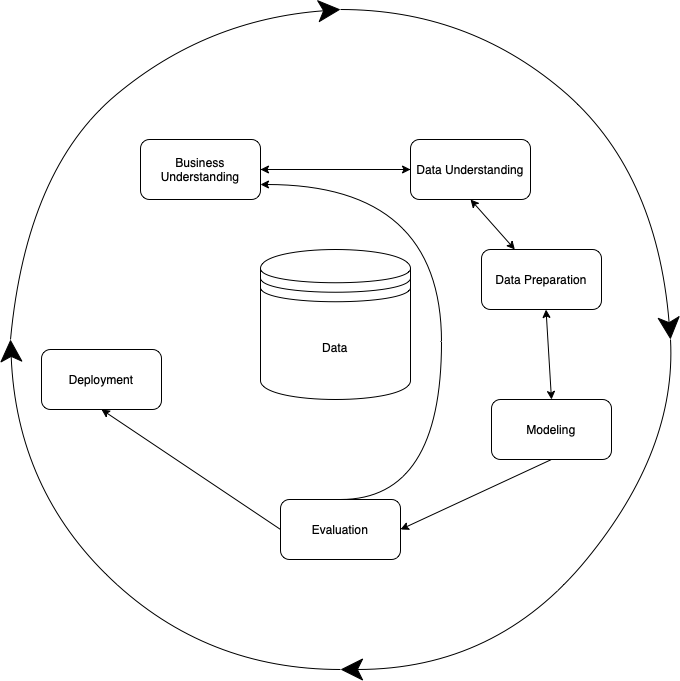
\includegraphics[width=0.7\textwidth]{./img/memoria/CRISP-DM}
\caption{Enfoque CRISP de la minería de datos~\cite{KOTU201517}.}
\label{./img/memoria/CRISP-DM}
\end{figure}

En~\cite{KOTU201517} se divide el proceso de la minería de datos en 5 etapas o pasos principales: establecimiento de los objetivos y comprensión del problema, recopilación y preparación de los datos, desarrollo del modelo, aplicación del modelo y la evaluación de los resultados y despliegue en producción. Ver Figura~\ref{fig:./img/memoria/machine-learning-pipeline}.

\imagen{./img/memoria/machine-learning-pipeline}{\textit{Machine Learning Pipeline}~\cite{mlpipeline2018}.}

\begin{enumerate}
   \item \textbf{Establecer los objetivos y comprensión del problema.}
    La primera etapa puede resultar la más complicada del proceso. Todas las partes interesadas deben de estar presentes y de acuerdo en la definición del problema que se va a tratar, esto incluye tanto a los científicos de datos como las terceras partes involucradas o interesadas. 
    Este procedimiento ayuda a la formulación de las preguntas de los datos y los parámetros a utilizar en el proyecto. Si se trata de un proyecto empresarial, se debe hacer un estudio o investigación adicional para comprender el contexto de la empresa.
    \item \textbf{Preparación de los datos.}
    Con el alcance del problema definido ya se puede comenzar a identificar qué conjunto de datos será el más efectivo o representativo con el fin de comenzar a dar respuesta a las preguntas formuladas en el proceso anterior.
    
    Una vez se dispone de todos los datos recogidos comienza el proceso de pre-procesado de los mismos. Este proceso se basa en la limpieza de los datos con el fin de eliminar cualquier posible ruido, entendiéndose por ruido los datos duplicados, los valores perdidos y aquellos atípicos; aquellos que puedan causar problemas a la resolución del problema o generen incertidumbre.
    En determinados conjuntos de datos se puede hacer una reducción de dimensiones. Consiste en la reducción del número de dimensiones que poseen las instancias recogidas, con el fin de eliminar aquellas que no sean realmente representativas o significativas, este proceso reduce la complejidad computacional\footnote{La cuantificación de la dificultad de un problema computacional en términos de recursos informáticos (como el tiempo de cálculo o la cantidad de memoria) necesarios para su solución.} de los cálculos posteriores. Por contrapartida hay que conocer cuáles serán los predictores con mayor relevancia en el problema para garantizar una precisión <<óptima>> del modelo.
    \item \textbf{Desarrollo del modelo.}
    Según~\cite{KOTU201517} el modelo es la representación abstracta de los datos y sus relaciones en un conjunto de datos concreto. Actualmente existen cientos de algoritmos que se pueden utilizar, habitualmente proceden de campos como la ciencia de datos, \textit{machine learning}, o la estadística.
    Se debe tener el conocimiento suficiente para entender cómo funciona el algoritmo para poder configurar correctamente los parámetros que este va a utilizar en base a los datos y el problema de negocio que estamos resolviendo. 
    
En función de cómo los modelos resuelven el problema se pueden clasificar en:
    \begin{enumerate}
        \item Regresión.
        \item Análisis de asociación.
        \item \textit{Clustering.}
        \item Detección de anomalías.
    \end{enumerate}
    
    El modelo debe ser creado con especial cuidado para evitar el \textit{overfitting}, \textit{i.e.} el modelo memoriza el conjunto de entrenamiento y no tendrá un rendimiento correcto una vez desplegado en producción. Se desea que el modelo sea lo más general posible de cara a \textit{aprender} de los datos del conjunto de entrenamiento.

    \item \textbf{Aplicación del modelo.}
	El momento de la aplicación del modelo es cuando de verdad se comprueba si realmente el modelo está listo para pasar al siguiente punto, en otras palabras, si es apto para ser desplegado en producción. 
	Para ello se tienen en cuenta métricas como la calidad del modelo ante el problema, su tiempo de respuesta, etc.
    
	\item \textbf{Evaluación de los resultados y despliegue en producción.}
	Es habitual que los parámetros con los que el modelo fue entrenado con el paso del tiempo dejen de ser los más interesantes, pudiendo ser comprobado el error proporcionado por el modelo con los datos de prueba. Cuando ese error sea excesivo o fuera de un margen dado se deberá de volver a entrenar el modelo, comprobar, y desplegar. 
	De esta forma se puede comprobar como el ciclo de vida del modelo es circular.
\end{enumerate}

El proceso aplicado en la minería de datos proporciona un marco de trabajo mediante el cual se permite extraer información aparentemente no trivial de grandes conjuntos de datos. 
Es un campo de aprendizaje constante, tanto el aplicar los conocimientos del analista para reducir las dimensiones del conjunto de datos, como una vez que se ha entrenado el modelo y puesto en producción, aprender los puntos fuertes de este y el porqué de éstos~\cite{Chapman2000CRISPDM1S}.

\subsection{Técnicas utilizadas en la minería de datos}

A continuación, se presentan una serie de técnicas utilizadas en función de la naturaleza de las instancias predictoras, y de la variable de salida. Si la variable o clase de salida es continua o categórica, nos encontramos con modelos de aprendizaje supervisado, mientras que, si no existe variable o clase de salida, nos encontramos con modelos de aprendizaje no supervisado~\cite{palmer2011data}.

\begin{enumerate}
	\item \textbf{Reglas de asociación} (además se trata de una técnica de aprendizaje automático). Se basa en el uso de reglas básicas utilizadas para localizar relaciones entre instancias en conjuntos de datos de gran tamaño. Para su correcto funcionamiento deben satisfacer el soporte (nivel) mínimo especificado por el usuario y la confianza o grado de satisfactibilidad especificada en tiempo constante.
	
	En determinadas ocasiones la generación de estas reglas es dividida en una serie de pasos:
	\begin{itemize}
	\item Para encontrar las $n$ instancias más frecuentes, se aplica un umbral mínimo, lo cual establece la información del conjunto de datos.
	\item Cuando el nivel mínimo de confianza es aplicable a aquellas instancias encontradas en el paso previo, se transforman en reglas. Este paso es el que más atención requiere.
	\end{itemize}
	\item \textbf{Redes neuronales.} Actualmente, principalmente utilizadas en \textit{deep learning}, simulan la interconectividad propia del cerebro humano utilizando capas de nodos. Cada nodo está compuesto por \(x_n\) entradas, \(w_n\) pesos y un sesgo o umbral, el cual al ser superado activa la neurona, pasando los datos del nodo a la siguiente neurona. El proceso es repetido a lo largo de $n$ iteraciones pasando el mismo conjunto de entrenamiento, conocido como \textit{epochs}.
	
	Las redes neuronales poseen tres ventajas en el uso de grandes conjuntos de datos: aprendizaje adaptado mediante ejemplos, robustez en el manejo de información redundante e imprecisa, y computación masiva paralela.
	\item \textbf{Árboles de decisión.} Se pueden definir como particiones secuenciales de un conjunto de datos, maximizando las diferencias a una variable dependiente. Ofrecen una forma concisa de definir grupos que son consistentes en sus atributos pero que varían en términos de la variable dependiente.
	
	Los árboles de decisión se encuentran compuestos de nodos (variables de entrada), ramas (grupos de variables de entrada), y hojas (valores de la variable de salida). La construcción de los árboles está basada en el principio de \textit{divide and conquer}, haciendo uso de un algoritmo de aprendizaje supervisado, se realizan divisiones sucesivas del espacio multi-variable con el objetivo de maximizar la distancia entre los grupos de cada división, \textit{i.e.} realizar particiones discriminatorias. El proceso de división finaliza cuando todas las entradas de una rama tienen el mismo valor en el nodo hoja, dando lugar al modelo completo. Cuanto más abajo estén las variables de entrada en el árbol, menos importantes son en la clasificación  de la salida.
	
	Para evitar el \textit{overfitting} del modelo, el árbol puede podarse eliminando las ramas con pocas instancias, o donde aquellas instancias sean poco representativas~\cite{palmer2011data}.
	
	Una de las principales diferencias sobre las redes neuronales y ventaja que poseen, es la interpretabilidad que ofrecen, ofreciendo una trazabilidad de la solución propuesta.
	
	\item \textbf{$k$-vecinos más cercanos. KNN (\textit{k-nearest neighbors})}~\cite{guo2003knn,hand2007principles,palmer2011data} Las técnicas \textit{k}-NN se basan en el concepto de similaridad. Permite la construcción de un método de clasificación sin hacer suposiciones sobre la forma de la función que relaciona la variable dependiente con las variables independientes.
	
	El objetivo es identificar de forma dinámica las \textit{k} instancias en los datos de entrenamiento que son similares (vecinas) a la instancia que se quiere clasificar. La clasificación de una instancia viene dada por la observación de la clase de la vecindad, para ello se basa en los atributos de las variables. En otras palabras, cuenta el número de instancias para cada clase en la vecindad y asigna a la instancia en cuestión aquella clase que sea mayoritaria en la vecindad~\cite{potomac1999introduction}.
	
	Asume que todas las instancias corresponden a puntos en un espacio $n$-dimensional. Pudiendo ser utilizado tanto en problemas de clasificación como de regresión.
\end{enumerate}

\section{Técnicas de selección de instancias}\label{sec:tecnicas-seleccion-instancias}
Dentro de los conjuntos de datos nos encontramos con las instancias, también llamadas ejemplos o prototipos, son cada uno de los elementos que componen el \textit{dataset}; en problemas reales de \textit{machine learning} es habitual que se requiera de clasificación automática de estos datos. Este proceso se puede llevar a cabo con algoritmos de aprendizaje supervisado, Sección~\ref{subsec:Aprendizaje-Supervisado}, con el objetivo de etiquetar la nueva información. Para poder hacerlo previamente se ha tenido que, entrenado el clasificador con un conjunto de entrenamiento, $T$~\cite{olvera2010review}.

En la práctica, cualquier $T$ dado contendrá información útil e información desechable, este último tipo de información --- que en realidad son instancias --- aparte de ser redundantes producen ruido, pudiendo inducir en una clasificación errónea en el proceso de aprendizaje, y posteriormente tener un modelo que no sea capaz de clasificar correctamente la nueva información.

\begin{figure}
\centering
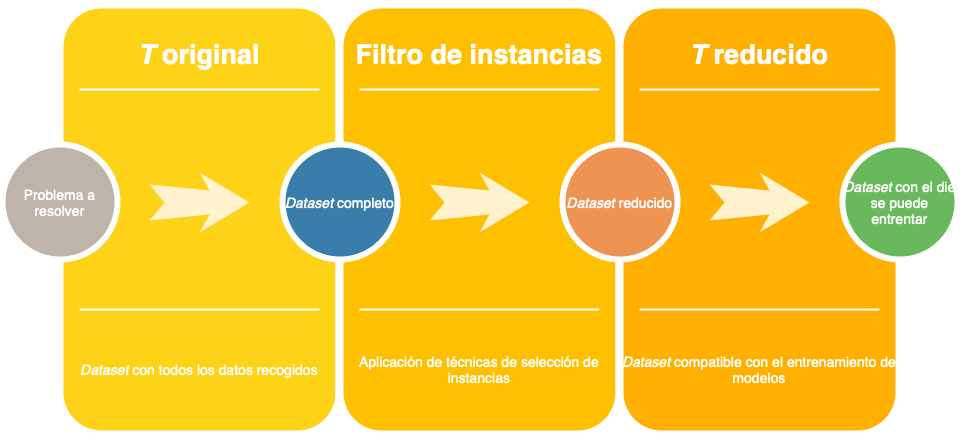
\includegraphics[width=\linewidth]{../img/memoria/Instance-Selection-Overview}
\caption{Proceso de selección de instancias.}
\label{fig:instance-election-overview}
\end{figure}

Es por ello por lo que un pre-procesado o \textbf{filtrado} de las instancias pertenecientes al $T$ original es necesario. En la Figura~\ref{fig:instance-election-overview} se ilustra de manera gráfica el proceso de selección de instancias. Dado un conjunto de datos de entrenamiento inicial, $T$, el objetivo será obtener un subconjunto $S$, tal que $S \subseteq T$ de manera que $S$ no contiene instancias redundantes ni <<ruidosas>>. Además, $Acc(S) \cong Acc(T)$, donde $Acc(X)$ es la precisión, \textit{accuracy} en inglés, del modelo entrenado con el conjunto de datos $X$.

En función de cómo comienzan a crear el nuevo subconjunto de datos, $S$, se identifican dos aproximaciones, ascendente y descendente.
\begin{itemize}
\item \textbf{Ascendente.} El nuevo conjunto de datos comienza estando vacío, $S = \emptyset$, y a medida que se vayan realizando iteraciones del algoritmo correspondiente, se irán añadiendo instancias a $S$. El principal problema que posee esta aproximación es su sensibilidad al orden, \textit{i.e.} dada una instancia $x \subset T$, en diferentes iteraciones del mismo algoritmo de selección de instancias sobre el mismo $T$, puede o no estar en $S$. Esto se debe a la aleatoriedad con la que se presentan los datos, para asegurar esta aleatoriedad los datos se escogen de manera aleatoria de $T$, intrínsecamente da una mayor facilidad a las muestras iniciales a estar en $S$ que las finales, ya que puede que ya se encuentren representadas o sean clasificadas como ruido.

Entre las principales ventajas de esta aproximación destaca el espacio de almacenamiento requerido, puesto que se van guardando instancias y por lo tanto en un inicio es muy pequeño.

\item \textbf{Descendente.} El nuevo conjunto de datos comienza siendo el conjunto de entrenamiento al completo, $S = T$, y a medida que se vayan realizando las iteraciones del algoritmo correspondiente, se irán eliminando instancias de $S$. Esta aproximación es mucho más costosa computacionalmente, para cada instancia que debe decidir si eliminar o no debe comprobar todo el subconjunto $S$, pero en contraposición consigue reducir más que la aproximación ascendente, el conjunto de entrenamiento $T$.
\end{itemize}

Junto con esta diferenciación, en función de la aproximación de selección de instancias se pueden distinguir dos agrupaciones.
\begin{itemize}
\item \textbf{\textit{Wrapper}.} El criterio de selección se basa en la precisión del clasificador. Aquellas instancias que no contribuyen a la mejora del clasificador se quedan fuera de $S$. Este trabajo está centrado en este criterio de selección.
\item \textbf{\textit{Filter}.} El criterio de selección utiliza una función, $f(x, y)$, para realizar la selección, no se basa en un clasificador concreto.
\end{itemize}

\begin{table}[]
\small
\begin{center}
	\begin{tabular}{lcc}
	\toprule 
	\textbf{Método}  &  \textbf{\begin{tabular}[]{@{}c@{}}Complejidad\\computacional\end{tabular}}  & \textbf{Referencia} \\
	\toprule
	\rowcolor[HTML]{EFEFEF} 
	Edición de Wilson (ENN)        & $O(n^2)$      &~\cite{wilson1972asymptotic}\\ 
	Condensado de Hart (CNN)     & $O(n^3)$         &~\cite{hart1968condensed}\\ 
	\rowcolor[HTML]{EFEFEF} 
	Condensado Reducido (RNN)     & $O(n^3)$         &~\cite{gates1972reduced}  \\ 
	\textit{Iterative Case Filtering} (ICF)     & $O(n^2)$              &~\cite{brighton2002advances}\\ 
	\rowcolor[HTML]{EFEFEF} 
	Subconjunto Selectivo Modificado (MSS)    & $O(n^2)$             &~\cite{barandela2005decision}\\ 
	\textit{Drecremental Reduction Optimization Procedure} (DROP) & $O(n^2)$  &~\cite{wilson2000reduction} \\ \bottomrule
	\end{tabular}
\end{center}
\caption{Resumen de la complejidad computacional de algunos métodos clásicos de selección de instancias.}
\label{tab:instance-selection-methods}
\end{table}

En la Tabla~\ref{tab:instance-selection-methods} se aprecian aquellos algoritmos implementados en primera instancia para la reducción de instancias dentro de $T$, el objetivo de todos ellos es que el subconjunto generado, $S$, sea capaz de clasificar correctamente  $T$ en su totalidad prácticamente.

\subsubsection{Algoritmos de selección de instancias}\label{subsubsec:Instance-Selection-Algorithms}
Existen multitud de algoritmos a día de hoy que son capaces de reducir el número de instancias de $T$, en este trabajo se van a comentar los pertenecientes a la Tabla~\ref{tab:instance-selection-methods}. Cada uno de ellos tiene sus ventajas y sus desventajas como cabe esperar, en la literatura no apreciamos un <<este es mejor que aquel>> o similar.

\paragraph{Algoritmo de edición de Wilson}\label{paragraph:ENN}
\hfill \break
Wilson~\cite{wilson1972asymptotic} (1972) publicó la regla del vecino más cercano editado, \textit{ENN}. Los problemas de clasificación de instancias en función de una etiqueta se caracterizan por:
\begin{itemize}
\item Hay una instancia a ser clasificada.
\item Existe un $S$ el cual posee instancias con la misma distribución que la instancia a clasificar, pudiendo ser comparables las instancias del conjunto con la que estamos analizando.
\item No existe información adicional del conjunto.
\item Existe una distancia medible entre instancias.
\end{itemize}

\begin{algorithm}[H]
	\KwIn{Conjunto de entrenamiento $X = \lbrace\left( x_1, y_1 ,\right)\dots \left(x_n, y_n\right)\rbrace$, $k$ número de vecinos.}
	\KwOut{Conjunto editado $S \subset X$}
  	\BlankLine
  	$S \leftarrow X$\\
  	\ForAll{$x \in S$}{
		Encontrar x.$N_{1\dots k+1}$, los $k$ + 1 vecinos más cercanos de $x \in X - \lbrace x \rbrace$\\
		\If{$\delta_{k-NN}\left(x_i\right)\neq \theta_i$}{
			Eliminar $x$ de $S$		
		}
  	}
  	\Return{$S$}
  \caption{Algoritmo de edición de Wilson, \textit{ENN}}\label{alg:Wilson-ENN}
\end{algorithm}

Con todas estas premisas Wilson propone un algoritmo basado en clasificación incorrecta en función de sus vecinos más cercanos. Cuando una instancia resulta mal clasificada por sus \textit{k} vecinos más cercanos, \textit{k}-NN, esa instancia es descartada. Finalmente obtendremos como resultado un conjunto $S$ con las instancias correctamente clasificadas por sus vecinos.

Suponiendo que sea \textit{X} un conjunto de \textit{N} instancias y \textit{M} posibles clases y, sea \textit{k} el número de vecinos cercanos, el algoritmo de Wilson se puede formular de la siguiente manera:

El algoritmo de edición de Wilson, ver algoritmo~\ref{alg:Wilson-ENN}, posee una complejidad computacional de $O(n^2)$. Una de las ventajas de este algoritmo es su forma de crear el subconjunto $S$, ya que al ser descendente las primeras iteraciones serán lentas --- dependiendo del tamaño de $T$ lógicamente --- pero las finales serán considerablemente más rápidas (siempre y cuando haya un nivel significativo de ruido).


\paragraph{Algoritmo Condensado de Hart}\label{paragraph:CNN}
\hfill \break
Hart~\cite{hart1968condensed} en 1968 propuso la que se considera la primera regla formal de condensador para NN. El algoritmo de condensado de Hart, \textit{CNN --- Condensed Nearest Neighbor}. Está basado en técnicas de consistencia y reducción. Sea $X \not= \emptyset$ y $S \subseteq X$, podremos decir que el subconjunto $S$ es consistente respecto al conjunto $X$ si al utilizar a $S$ como conjunto de aprendizaje, se puede clasificar correctamente a todo el conjunto $X$.

El algoritmo de Hart es una técnica ascendente, a partir de las primeras instancias que se añadan a $S$ se clasificarán y añadirán, o no, a $S$. Consiste en encontrar entre todas las instancias de $T$ un subconjunto $S$ tal que cada instancia de $T$ sea más cercano a las instancias en $S$ de su misma clase que a las instancias de otras clases, permitiendo utilizar $S$ como conjunto de clasificación de $T$. Para el correcto funcionamiento se asume que el conjunto $T$ es consistente, no posee dos instancias idénticas con pertenencia a diferentes clases.

El algoritmo propuesto por Hart~\cite{hart1968condensed}, ver algoritmo~\ref{alg:Hart-CNN}, posee una complejidad computacional de $O(n^2)$. El conjunto obtenido a partir de $T$, \textit{i.e.} $S$, operando con grandes conjuntos de datos demuestra poseer un tamaño considerablemente menor respecto a $T$. 

Si bien es una técnica utilizada por su efectividad, posee una serie de puntos negativos a su vez.
\begin{itemize}
\item Sensibilidad ante el ruido. Un objeto ruidoso no será correctamente clasificado por sus vecinos. Estas muestran no se eliminarán del conjunto solución $S$, por lo que no desaparecerán.
\item $S$ no tiene por qué ser el menor conjunto de $T$. Diferentes ejecuciones del algoritmo sobre el mismo $T$ pueden dar diferentes conjuntos solución $S$. Esto se debe al orden aleatorio por el cual se seleccionan las instancias. Por definición del propio algoritmo se asume que no se va a alcanzar de forma general el subconjunto de tamaño mínimo que cumpla con las características especificadas.
\end{itemize}

\begin{algorithm}[H]
	\KwIn{Conjunto de entrenamiento $X$}
	\KwOut{Conjunto editado $S \subset X$}
  	\BlankLine
  $S \leftarrow \left\lbrace x_1 \right\rbrace$\\
  	\ForAll{$x \in S$}{
		\If {$x$ no se clasifica correctamente usando $S$}{
			Añadir $x$ a $S$\\
			Reiniciar
		}
  	}
  	\Return{$S$}
	\caption{Algoritmo Condensado de Hart, \textit{CNN}.}\label{alg:Hart-CNN}
\end{algorithm}

\paragraph{Algoritmo Condensado Reducido}\label{paragraph:RNN}
\hfill \break
Gates~\cite{gates1972reduced} en 1972 propuso el algoritmo del conjunto reducido, basado en las reglas \textit{NN}. El algoritmo propuesto es una modificación del algoritmo \textit{CNN}, ver algoritmo~\ref{alg:Hart-CNN}. No es una nueva regla de decisión puesto que se sigue eligiendo la clase del vecino más cercano para la clasificación. 
El algoritmo se basa en un procedimiento para seleccionar el subconjunto $T_{CNN}$, el cual debe comportarse igual de bien que $T_{NN}$ ante clasificaciones de instancias desconocidas. Como se puede apreciar en el propio algoritmo~\ref{alg:Gates-RNN}, puede existir una disminución del rendimiento, a cambio se obtiene una mejora de la eficiencia para el algoritmo de clasificación que posteriormente se utilice, tanto en la cantidad de memoria utilizada como en el tiempo de computación.

De igual manera que en \textit{CNN}, posee la problemática de la minimalidad, si bien el conjunto resultante $S \subset T$ será consistente, no se puede asegurar que sea mínimo; y diferentes ejecuciones del algoritmo sobre el mismo conjunto de datos $T$, pueden obtener diferentes subconjuntos solución~$S$.

\begin{algorithm}[H]
	\KwIn{Conjunto de entrenamiento $X$}
	\KwOut{Conjunto editado $S \subset X$}
  	\BlankLine
  $S \leftarrow \left\lbrace x_1 \right\rbrace$\\
  	\ForAll{$x \in S$}{
		\If {$x$ no se clasifica correctamente usando $S$}{
			Añadir $x$ a $S$\\
			Reiniciar
		}
  	}
  	\ForAll {$x \in S$}{
			Eliminar $x$ de $S$\\
		\If {$\exists x_i$ incorrectamente clasificada usando $S$}{
			Añadir $x$ a $S$
		}
	}
  	\Return{$S$}
	\caption{Algoritmo Condensado Reducido, \textit{RNN}.}\label{alg:Gates-RNN}
\end{algorithm}

\paragraph{Algoritmo \textit{Iterative Case Filtering}}\label{subsubsub:ICF}
\hfill \break
Brighton~\cite{brighton2002advances} en 2002 propuso el algoritmo iterativo de filtrado, \textit{ICF}, bajo la premisa de predecir la clase de una instancia con la misma precisión, o mayor si fuera el caso, que el $T$ original. Uno de los objetivos principales del propio algoritmo es mantener en el subconjunto $S$ únicamente aquellas instancias que sean críticas para la decisión.

\textit{ICF} utiliza una estrategia decremental, \textit{i.e.} de manera iterativa va borrando instancias del conjunto de datos inicial, inicialmente realiza un filtrado y posteriormente la reducción~\cite{brighton2002advances} Al reducir el tamaño de $T$ los tiempos de respuesta para el proceso de clasificación mejorarán, ya que se examinarán un menor número de instancias para realizar la clasificación; por contrapartida al eliminar muestras que se creen que son dañinas para el proceso, se pueden estar eliminando algunas que sean clave y por lo tanto teniendo una degradación de la calidad del clasificador.

\textit{ICF} se basa en dos categorías para la decisión de si una instancia debe permanecer o no en $S$, ver algoritmo~\ref{alg:Brighton-ICF}, estas son \textit{Coverage} y \textit{Reachable}. Definidas de la siguiente manera para el caso base $\mathcal{CB} = \lbrace x_1, x_2, ..., x_n\rbrace$.
\begin{align*}
Coverage (x) = \lbrace x' \in \mathcal{CB} : Adaptable(x, x')\rbrace  \\
Reachable (x) = \lbrace x' \in \mathcal{CB} : Adaptable(x',x)\rbrace
\end{align*}

Una instancia $x$ podrá estar en el conjunto adaptable de $x'$ sí y solo si $x$ es una instancia relevante para la solución de $x'$, \textit{i.e.} $x \in k-NN(x)$. La problemática surge en el momento en el cual una instancia con clase diferente no permite la correcta clasificación de $x'$, es por ello por lo que el vecindario de $x'$ viene definido por todas las instancias antes de la primera instancia de diferente clase, utilizando \textit{sets} descritos por Wilson y Martinez. La propiedad \textit{Reachable} no está fijada desde el principio del algoritmo, sino que es dinámica siendo fijada cada vez en función de la instancia de clase diferente más cercana. El criterio seguido para realizar la eliminación de una muestra es: si el \textit{set} formado por el $reachable(x)$ es mayor que el $coverage(x)$, \textit{i.e.} una instancia $x$ es eliminada cuando más instancias pueden resolver $x$ que las que $x$ puede resolver por sí misma.

\begin{algorithm}[H]
	\KwIn{Conjunto de entrenamiento $X$}
	\KwOut{Conjunto editado $T \subset X$}
  	\BlankLine
  \tcc{Filtro de ruido en función de la regla \textit{k-NN}}
  $T \leftarrow ENN(X,k)$\\  	
  \Repeat{no $progress$}{
  		\ForAll {$x \in T$}{  
  			Calcular $coverage(x)$\\
  			Calcular $reachable(x)$
  		}
  		$progress \leftarrow$ \textbf{false}\\
  		\ForAll {$x \in T$}{
			\If {$\left| reachable(x) \right| > \left| coverage(x) \right|$}{
				Marcar $x$ para eliminar\\
				$progress \leftarrow $ \textbf{true}
			}
		}
		\ForAll {$x \in T$}{
			\If{$x$ marcada para eliminar}{
				Eliminar $x$ de $T$
			}
		}
  }
  	\Return{$T$}
	\caption{\textit{Iterative Case Filtering}, \textit{ICF}.}\label{alg:Brighton-ICF}
\end{algorithm}

\paragraph{Algoritmo Subconjunto Selectivo}\label{paragraph:SS}
\hfill \break
Ritter~\cite{ritter1975algorithm} 1975 propone un algoritmo capaz de satisfacer la condición de consistencia del algoritmo condensado de Hart, ver algoritmo~\ref{alg:Hart-CNN}; para ello introduce una condición más <<fuerte>> de consistencia, el objetivo es encontrar aquellas instancias de un orden independiente. 

Un subconjunto $S$ del conjunto de entrenamiento $T$, es un Subconjunto Selectivo, $SS$, si $SS$ cumple las siguientes condiciones:
\begin{enumerate}
\item El subconjunto $S$ debe ser consistente.
\item Todas las instancias tienen que ser más cercanas a un vecino selectivo de la misma clase que a cualquier otra instancia de otra clase.
\item No puede haber ningún subconjunto $S'$ que satisfaga las condiciones 1 y 2, y que al mismo tiempo contenga un menor número de instancias que el Subconjunto Selectivo, $SS$.
\end{enumerate}

La segunda condición es la diferencia principal entre el algoritmo de Hart y el subconjunto calculado con el algoritmo del subconjunto selectivo. De forma que se puede re-formular el punto número dos de la siguiente manera:

\emph{Todas las instancias del conjunto de entrenamiento $T$ deben de ser más cercanos a un vecino condensado --- miembro del subconjunto condensado $\mathcal{CS}$ --- de la misma clase que a cualquier otra instancia de otra clase diferente del $\mathcal{CS}$.}

Pudiendo verse como una reformulación del punto nº 1. Además, el punto nº  2 para el subconjunto selectivo permite un subconjunto de menor tamaño, eliminando la necesidad de calcular todas las permutaciones de las instancias en $T$. Con unos criterios más específicos que los que se encuentran en el algoritmo condensado, el subconjunto selectivo resultante no tiene por qué ser mínimamente consistente. Asimismo, de forma general, no será un subconjunto reducido del $S$ producido por \textit{CNN}.


\paragraph{Algoritmo Subconjunto Selectivo Modificado}\label{paragraph:MSS}
\hfill \break
Barandela~\cite{barandela2005decision} 2005 propuso el algoritmo de subconjunto selectivo modificado, \textit{MSS}, como su propio nombre indica, se trata de una modificación del algoritmo Subconjunto Selectivo, SS. Debido a que no se puede garantizar que el algoritmo de Ritter~\cite{ritter1975algorithm} devuelva un subconjunto, $S$, el cual sea mínimo y consistente, habiendo sido categorizado como un problema NP-Completo~\cite{wilfong1992nearest}, por lo que \textit{MSS} pretende conseguir el subconjunto mínimo consistente mediante el uso de la propiedad selectiva.

La aproximación realizada por Barandela \textit{et al.} modifica la condición nº 3 anteriormente propuesta, mientras que las nº 1 y 2 no son modificadas. De forma que la definición nº 3 queda formulada de la siguiente manera:

\emph{El Subconjunto Selectivo Modificado, \textit{MSS}, se define como el subconjunto del conjunto de entrenamiento $TS$, el cual $\forall x_i \in TS$ aquella instancia de $Y_i$ que es más cercano a otra clase que a la de $x_i$, \textit{i.e.} el más cercano a su enemigo más cercano.}


El objetivo principal de esta modificación es reforzar la condición que debe cumplir el subconjunto reducido para maximizar la aproximación a la frontera de decisión. Quedando definido el algoritmo, ver algoritmo~\ref{alg:Barandela-MSS}, como una alternativa eficiente al algoritmo propuesto por Ritter \textit{et al.}, siendo capaz de seleccionar mejores instancias (más cercanas a la frontera de decisión). 

El criterio que sigue \textit{MSS} para determinar la frontera de decisión es la distancia al enemigo más cercano. Con esta medida se puede definir el mejor subconjunto selectivo como aquel que contiene el mejor vecino relacionado para cada instancia en el $TS$. (Será mejor cuanto menor distancia a su enemigo más cercano posea).

\begin{algorithm}[H]
	\KwIn{Conjunto de entrenamiento $X$}
	\KwOut{Conjunto editado $S \subset X$}
  	\BlankLine
  $S \leftarrow \emptyset$\\  	
  Ordenar las instancias $\lbrace x_i \rbrace^{n}_{i=1}$ en función de $D_i$ a su enemigo más cercano\\
  \For {$i = 1$ hasta $n$}{
		$add \leftarrow$ \textbf{false}\\
		\For {$j=i$ hasta $n$}{
			\If {$x_j \in T \bigwedge d\left( x_i, x_j \right) < D_j$}{
				 Eliminar $x_j$ de $T$\\
				 $add \leftarrow$ \textbf{true}
			}
		}
		\If {$add$}{
			Añadir $x_i$ a $S$
		} 
		\If {$T = \emptyset$}{
			\textbf{return} $S$
		}
	}
	\caption{\textit{Modified Selective Subset}, \textit{MSS}.}\label{alg:Barandela-MSS}
\end{algorithm}

\paragraph{\textit{Decremental Reduction Optimization Procedure}}\label{paragraph:DROP}
\hfill \break
Bajo el nombre de \textit{Decremental Reduction Optimization Procedure, DROP}~\cite{wilson2000reduction} nos encontramos con hasta 5 aproximaciones para la resolución del mismo problema. Todas ellas seleccionan prototipos en función de \textit{socio} y \textit{asociado}. Definidos como:
\begin{itemize}
\item Socio. Sea $X \not= \emptyset$, el socio de un objeto $P$ el cual pertenece al conjunto $X$, es aquél objeto que tiene a $P$ como uno de sus $k$ vecinos más cercanos.
\item Asociado. Todo prototipo que contenga a $P$ como a uno de sus $k$ vecinos más cercanos, será denominado asociado de $P$, denotado con la expresión $P.A_{1,\dots,a}$ donde $a$ es el número de asociados de $P$.
\end{itemize}

Volviendo sobre los conceptos de \textit{coverage} y \textit{reachable} vistos en el algoritmo \textit{Iterative Case Filtering}, (ICF), podemos relacionar todos los conceptos de la siguiente manera: los asociados de un prototipo $P$ se pueden ver como el conjunto formado por el \textit{reachable} de $P$, y con el \textit{coverage} se pueden obtener los socios del prototipo $P$.

Todas las aproximaciones de $DROP\lbrace 1\dots5\rbrace$ se basan en el mismo algoritmo~\cite{wilson2000reduction} pero con modificaciones en las técnicas de pre-procesado de los prototipos. Sus diferencias son:
\begin{itemize}
\item \textit{DROP1}. Eliminará un objeto $P$ de $S$ si sus socios en $S$ se clasifican correctamente sin $P$, \textit{i.e.} la ausencia de $P$ no impide la correcta clasificación del resto de prototipos.
\item \textit{DROP2}. Eliminará un objeto $P$ de $S$ si los socios que tiene $P$ en $TS$ se clasifican correctamente sin $P$, \textit{i.e.}, verificará el efecto que causa esta eliminación sobre la muestra original. Previo al proceso de eliminación de objetos $P$, ordena los prototipos a tratar en orden a su enemigo más cercano, permitiendo que los primeros prototipos que se van a tratar serán aquellos más alejados de las fronteras de decisión, ergo las más prescindibles.
\item \textit{DROP3}. Lo primero de todo realiza un filtrado de ruido, para ello aplica la edición de Wilson, ver algoritmo~\ref{alg:Wilson-ENN}. Seguidamente aplica el algoritmo \textit{DROP2}, ver algoritmo~\ref{alg:DROP3}.
\item \textit{DROP4}. Aplica un filtro de ruido diferente, en este caso consistirá en eliminar un prototipo solo si su eliminación no provoca que alguna otra instancia sea mal clasificada.
\item \textit{DROP5}. Modificación sobre \textit{DROP2}, en este algoritmo el proceso de eliminación de objetos comienza por aquellos más cercanos a sus enemigos. 
\end{itemize}

El concepto \textit{with} permite recoger el número de asociados correctamente clasificados teniendo en cuenta un prototipo $x$ como vecino, en cambio \textit{without} tiene en cuenta el número de asociados correctamente clasificados los cuales no tienen el prototipo $x$ como vecino. En los casos en los que $without > with$ se está tratando con un prototipo el cual no aporta información sobre el conjunto $S$ permitiendo su eliminación.

\begin{algorithm}[H]
	\KwIn{Conjunto de entrenamiento $X$ y número de vecinos más cercanos a considerar, $k$}
	\KwOut{Conjunto editado $S \subset X$}
  	\BlankLine
  $S \leftarrow \text{Filtrado de ruido}(X)$ \\
	Ordenar las instancias de $S$ por la distancia a su enemigo más próximo \tcc*[f]{de mayor a menor}\\
	\ForAll{$x \in S$}{
		Encontrar los $x.N_{1\dots k+1}$, los $k+1$ vecinos más cercanos de $x$ en $S$\\
		Añadir $x$ a la lista de asociados de cada uno de sus vecinos
	}
	\ForAll{$x \in S$}{
		$with \leftarrow$ número de asociados de $x$ clasificados correctamente \textbf{con} $x$ como vecino\\
		$without \leftarrow$ número de asociados de $x$ clasificados correctamente \textbf{sin} $x$ como vecino\\
		\If{$without \geq with$}{
			Eliminar $x$ de $S$\\
			\ForAll{Asociado $a$ de $x$}{
				Eliminar $x$ de la lista de vecinos de $a$\\
				Encontrar nuevo vecino para $a$\\
				Añadir $a$ en la lista de asociados del nuevo vecino
			}
		}
	}
	\Return{$S$}
	\caption{\textit{Decremental Reduction Optimization Procedure 3}, \textit{DROP3}.}\label{alg:DROP3}
\end{algorithm}

\section{Función distancia entre instancias}
Una función distancia proporciona información sobre la proximidad entre dos instancias en función de todos sus parámetros. Si la distancia que separa dos instancias es cero, ambas instancias son idénticas. Se tiende a trabajar con conjuntos de datos normalizados, \textit{i.e.} todos los datos son ajustados a una escala común, independientemente de la escala en la que hayan sido medidos, para evitar que atributos/características con mucha varianza puedan <<despistar>> a los algoritmos.

Existen multitud de métricas para calcular la distancia, pudiendo variar la distancia calculada en función de cuál se aplique. Se van a comentar las más representativas.
\begin{itemize}
\item \textbf{Distancia de Minkowski.} La distancia de Minkowski es una métrica en el espacio vectorial normalizado. Es una métrica que se puede modificar con facilidad para calcular la distancia entre dos instancias de diferentes maneras. 
\begin{enumerate}
\item \(p = 1\), cálculo de la distancia de Manhattan.
\item \(p = 2\), cálculo de la distancia Euclídea.
\item \(p = \infty\), cálculo de la distancia de Chebyshov.
\end{enumerate}
Su fórmula es la siguiente:
\[ \mathbb{D}(x, y) = \left( \sum_{i=1}^{n}\left| x_i - y_i \right|^p \right)^{1/p} \]

\item \textbf{Distancia de Manhattan} o distancia del taxista. Es una métrica en un espacio vectorial normalizado, calculándose como la suma de los $n$ segmentos verticales u horizontales que unen dos puntos.

Su fórmula es la siguiente:
\[  \mathbb{D}(x, y) = \sum_{i=1}^{d}\left| x_i - y_i\right| \]

\item \textbf{Distancia euclidiana} o norma L2 o distancia L2. Es la distancia en línea recta entre dos puntos de datos en el espacio euclidiano.

Su fórmula normalizada es la siguiente:
\[  \mathbb{D}(x, y) = \sqrt{\sum_{i=1}^{d} \frac{\left(x_i - y_i\right)^2}{\sigma_i^2}}  \]

\item \textbf{Distancia de Chebyshov} o distancia del tablero de ajedrez. La distancia entre dos puntos es la mayor de sus diferencias a lo largo de cualquiera de sus dimensiones coordenadas.

Su fórmula es la siguiente:
\[  \mathbb{D}(x, y) = \max_i\left(\left|x_i - y_i\right|\right) \]

\end{itemize}

\capitulo{4}{Técnicas y herramientas}

En este capítulo se van a comentar las técnicas y herramientas utilizadas a lo largo del desarrollo del proyecto \textit{software}.

\section{Técnicas}\label{sec:tecnicas}

\subsection{Metodología SCRUM}\label{SCRUM}
\textit{Scrum} es un marco de trabajo que permite el trabajo colaborativo en equipos. Permite que los equipos que trabajan en proyectos con esta metodología se organicen por sí mismos, siendo ellos los que deciden cómo afrontar los problemas que van surgiendo. 

Según \cite{cervone2011understanding}, el modelo \textit{Scrum} se basa en tres componentes principales: roles, procesos y artefactos. El \textit{Scrum Master} es el puesto asumido por el director o gerente del proyecto, o en algunos casos el líder del equipo. Esta figura representa los valores y principios por los que se rige la metodología de \textit{scrum}, manteniendo los valores y buenas prácticas, así como resolviendo los impedimentos que vayan surgiendo a lo largo del desarrollo del proyecto. Habitualmente los equipos están compuestos por entre cinco y diez personas que trabajan en el proyecto a tiempo completo. Siendo este equipo independiente y flexible en cuanto a jerarquía interna, no siendo representado el papel del <<jefe>> dentro de este por la misma persona siempre. Esto genera que el papel cambie en función de las necesidades del propio proyecto, la configuración del equipo cambia únicamente entre iteraciones, o \textit{sprints}, no dentro de los mismos.

\begin{figure}[]
	\centering
	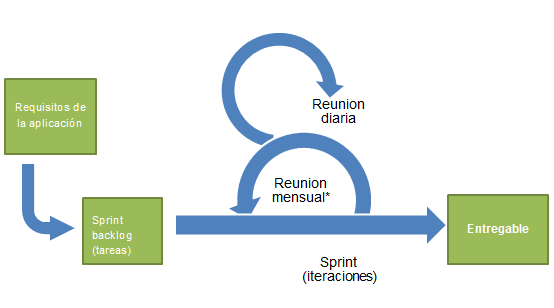
\includegraphics[scale=0.5]{../img/anexos/scrum-overview-es}
	\caption{Metodología \textit{scrum}~\cite{SCRUMWIKI}.}\label{img:scrum-overview}
\end{figure}

\subsubsection{\textit{Sprints}}
Los \textit{sprints} son periodos breves de \textbf{tiempo fijo} en el que el equipo trabaja para completar una cantidad de trabajo pre-establecida. Si bien muchas guías asocian los \textit{sprints} a la metodología ágil, asociando la metodología ágil y la metodología seguida en \textit{scrum} como si fueran lo mismo, cuando no lo son. La metodología ágil constituye una serie de principios, y la metodología \textit{scrum} es un marco de trabajo con la única finalidad de conseguir resultados.

A pesar de las similitudes los \textit{sprints} poseen un objetivo subyacente, entregar con frecuencia \textit{software} de trabajo.

\subsubsection{\textit{Sprint meetings}}
Dentro de la metodología \textit{scrum} existen diferentes reuniones que favorecen la agilidad del proyecto y que todo el mundo sepa lo que tiene que hacer en cada momento.
\begin{itemize}
\item \textbf{\textit{Sprint planning meeting.}} Esta reunión puede tener una duración de hasta de un día completo de trabajo. En ella deben de estar presentes todas las partes del proyecto, \textit{i.e.} el \textit{Scrum Master}, el equipo de desarrollo, y el \textit{product owner}. Poseen dos partes, en la primera de ellas se define el \textit{product backlog}, requerimientos del proyecto y se definen los objetivos para el \textit{sprint} que comienza, \textit{i.e.} lo que se espera ``construir'' o completar en el \textit{sprint}. En la segunda parte de la reunión se trabaja en el \textit{sprint backlog}, las tareas que se van a seguir en el \textit{sprint} para completar el objetivo de éste.
\item \textbf{\textit{Daily meeting.}} Debido a que los requerimientos del proyecto no se pueden variar durante la vida de un \textit{sprint}, existen las reuniones diarias que son organizadas por el \textit{Scrum Master} en las que se comenta el trabajo del día previo, lo que se espera de ese día y qué está retrasando o impidiendo a un individuo el proseguir con sus tareas, esta reunión no debe tener una duración de más de quince minutos y se debe realizar ``de pie''. No es una reunión para ver quién retrasa el proyecto sino para ayudar a quién lo necesite entre todos los miembros del equipo y permitir esa agilidad.
\item \textbf{\textit{Sprint review meeting.}} Reunión fijada al final de cada \textit{sprint} en la cual se hace una puesta en conocimiento de lo que se ha realizado en ese \textit{sprint}, siempre que se pueda se hará una demostración funcional en lugar de una presentación al \textit{product owner}. Esta reunión tiene un carácter informal.
\end{itemize}
 
\subsubsection{Artifacts}
Uno de los componentes más importantes de cara a la metodología \textit{scrum} son los artefactos, o \textit{artifacts} por su nombre en inglés. Éstos incluyen el \textit{product backlog}, el \textit{sprint backlog} y los \textit{burn down charts}.
\begin{itemize}
\item \textbf{\textit{Product backlog.}} Lista de trabajo ordenada por las prioridades para el equipo de desarrollo. Es generada a partir de las reuniones de planificación de los \textit{sprints}, contiene los requisitos. Se encuentra actualizado y clasificado en función de la periodicidad asignada a las tareas, pudiendo ser de corto o largo plazo. Aquellas tareas que se deban resolver a corto plazo deberán estar perfectaemnte descritas antes de asignarlas esta periodicidad, implicnddo que se han diseñado las historias de usuario completas así como el equipo de desarrollo ha establecido las estimaciones correspondientes. Los elementos a largo plazo pueden ser abstractos u opacos, conviene que estén estimados en la medida de lo posible para poder tener en cuenta el tiempo que llevará desarrollarla.

Los propietarios del producto dictan la prioridad de los elementos de trabajo en el \textit{product backlog}, mientras que el equipo de desarrollo dicta la velocidad a la que se trabaja en \textit{backlog}~\cite{danradigan2021}.

La estimación es una parte muy importante ya que es lo que permitirá al equipo de desarrollo mantener el ánimo y el trabajo al ritmo deseado. La estimación es realizada en la \textit{sprint planning meeting}, en la que se estima para cada tarea/producto del \textit{product backlog}. No se busca tener un resultado exacto del tiempo que va a llevar al equipo completar esa tarea, sino es una previsión. Para realizar correctamente la estimación se debe tener en cuenta el tamaño y la categoría de la tarea, los puntos de historia que se le van a asignar, así como el número de horas y días que van a ser necesarias para completar la tarea. 

\item \textbf{\textit{Sprint backlog.}} Lista de tareas extraídas del \textit{product backlog} que se han acordado desarrollarse a lo largo de un \textit{sprint}. Este \textit{backlog} es seleccionado por el propio equipo de desarrollo, para ello seleccionan una tarea del \textit{product backlog} y se divide en tareas de menor tamaño y abordables. Aquellas tareas de menor tamaño que el equipo no haya sido capaz de desarrollar previo a la finalización del \textit{sprint} quedarán almacenadas para próximos \textit{sprints} en el \textit{sprint backlog}.
\end{itemize}

\subsubsection{Actores, roles y responsabilidades}
Dentro de un equipo que sigue la metodología \textit{scrum} encontramos diferentes actores, como ya se ha comentado el equipo de desarrollo suele estar compuesto por entre cinco y diez personas, además del \textit{Scrum Master} y el \textit{Product Owner}~\cite{julioroche_2020}.
\begin{itemize}
\item \textbf{\textit{Product Owner.}} Encargado de optimizar y maximizar el valor del producto, es la persona encargada de gestionar las prioridades del \textit{product backlog}. Una de sus principales tareas es la de intermediario con los \textit{stakeholders}, partes interesadas, del proyecto; junto con recoger los requerimientos de los clientes. Es habitual que esta figura sea representante del negocio, con lo que aumenta su valor.

Para cada \textit{sprint} debe de marcar el objetivo de éste de manera clara y acordada con el equipo de desarrollo, lo cual hará que el producto vaya incrementando constantemente su valor. Para que todo fluya como debe, esta figura tiene que tener el ``poder'' de tomar decisiones que afecten al producto.

\item \textbf{\textit{Scrum Master.}} Figura con dos responsabilidades, gestionar el proceso \textit{scrum} y ayudar a eliminar impedimentos que puedan afectar a la entrega del producto.
\begin{enumerate}
\item Gestionar el proceso \textit{scrum}. Su función es asegurarse de que el proceso se lleva a cabo correctamente, facilitando la ejecución de éste y sus mecánicas. Consiguiendo que la metodología sea una fuente de generación de valor.
\item Eliminar impedimentos. Eliminar los problemas que vayan surgiendo a lo largo de los \textit{sprints} con el fin de mantener el ritmo de trabajo dentro de los equipos de desarrollo para poder entregar valor, manteniendo la integridad de la metodología.
\end{enumerate}
\item \textbf{Equipo de desarrollo.} Formado por entre cinco y diez personas encargados del desarrollo del producto, organizados de forma autónoma para conseguir entregar las tareas del \textit{product backlog} asignadas al \textit{sprint} correspondiente. Para que funcione correctamente la metodología todos los integrantes deben de conocer su rol dentro del equipo, internamente se pueden gestionar como el equipo considere, pero de cara <<hacia fuera>> son un equipo con una responsabilidad.
\end{itemize}

\subsection{Python}
Según~\cite{queespython}, Python es un lenguaje de programación multiplataforma y multiparadigma\footnote{Debido a que soporta parcialmente la orientación a objetos, la programación imperativa, y la programación funcional.}, entre sus principales características se encuentran la legibilidad y limpieza del código. Python es \textit{open source software} por lo que su uso es gratuito~\cite{pythonLICENSE}.

Python fue desarrollado al principio de la década de 1990 por Guido van Rossum en el Stichting Mathematish Centrum, CWI, en el Reino de los Países Bajos. Implementado como el sucesor del lenguaje ABC. Actualmente el lenguaje sigue siendo desarrollado por Guido, junto con contribuciones de muchos otros. El lenguaje está fuertemente influenciado por otros como: ABC, Ada, ALGOL 68, APL, C, C++, CLU, Dylan, Haskell, Icon, Java, Lips, Modula-3, Perl, Standard ML.

El principal objetivo de Python es la automatización de procesos con el fin de minimizar tanto complicaciones como tiempo de desarrollo. Debido a estas dos características, a día de hoy Python es el lenguaje de programación más utilizado para desarrollo de todo tipo de aplicaciones, tanto es así que, según las últimas estadísticas recuperadas por PYPL, ver~\cite{pyplindex}, además es el lenguaje de programación sobre el que más tutoriales se buscan en el top buscadores (Google, Bing, DuckDuckGo,\dots). Se aplica en campos tales como:
\begin{itemize}
\item Ciencia de datos. Uso de las bibliotecas de Python desarrolldas para el análisis y visualización de datos.
\item Aprendizaje automático. Dado que Python es un lenguaje de programación tan estable, flexible y sencillo, es perfecto para varios proyectos de aprendizaje automático (ML) e inteligencia artificial (AI). De hecho, Python es uno de los lenguajes favoritos entre los científicos de datos, y hay muchas bibliotecas y paquetes de aprendizaje automático e IA disponibles en Python. 
\item Desarrollo web. Utilizado principalmente en el \textit{back-end} de las aplicaciones web, tanto en la codificación de las funcionalidades, de manera similar a lo que JavaScript permitiría hacer; como encargándose de la conexión con las diferentes bases de datos que puedan estar en producción.
\item Visión artificial y procesamiento de imágenes. 
\item Desarrollo de videojuegos.
\item Medicina y bioinformática.
\item Astronomía.
\end{itemize}

\subsubsection{PEP8}
La abreviación PEP hace referencia a \textit{Python Enterprise Proposal}~\cite{pep8javatpoint}. La escritura de código con la lógica adecuada en un factor clave independientemente del lenguaje de programación en el que se esté trabajando, pero hay muchos más factores que influyen en la calidad del código. El estilo de codificación del programador hace que el código sea mucho más fiable, se debe de tener en cuenta que Python sigue estrictamente la forma de orden y formato de la cadena, \textit{i.e.} tal y como se escribe el código se procesa para su compilación.

PEP8 es un documento el cual proporciona varias directrices para escribir la parte legible en Python. Fue escrito oficialmente en 2001 por Guido van Rossum, Barry Warsaw y Nick Coghlan, con el objetivo principal de mejorar la legibilidad y consistencia del código. Disponible para consulta~\cite{rossum_warsaw_coghlan}.

PEP8 mejora la legibilidad del código, pero, ¿a qué se debe que la legibilidad sea tan importante en Python? <<\textit{Code is much more often than it is written.}>>~\cite{guidophrase}. Un fragmento de código puede ser escrito en cuestión de minutos o unas pocas horas, pero una vez escrito no se reescribirá nunca, pero seguramente sí que será leído un número indefinido de veces. Es en ese preciso momento cuando se debe tener una idea del por qué de esa línea de código. El código debe reflejar el significado de cada línea, de ahí el motivo de que la legibilidad sea tan importante.


\section{Herramientas}\label{sec:herramientas}
\subsection{UBUMLaaS}\label{UBUMLaaS}
UBUMLaaS surge como una plataforma de \textit{Machine Learning as a Service} basada en los métodos desarrollados tanto por el grupo de investigación ADMIRABLE\footnote{\textit{Advanced Data MIning Research And (Business intelligence | Bioinformatics | Big data) LEarning}.  El objetivo principal del grupo de investigación es el desarrollo de nuevos algoritmos de \textit{ensemble} y la aplicación de técnicas de minería de datos y \textit{pattern matching} a diversos campos como la bioinformática, la clasificación de series temporales y el análisis de datos de alta dimensión~\cite{admirable_intro}}. Junto con los desarrollados por BEST-AI\footnote{El Grupo de Investigación BEST-AI (Biología, Educación y Salud con Tecnologías Avanzadas Informáticas) de la Universidad de Burgos, centra su actividad investigadora en el desarrollo de nuevos algoritmos de minería de datos e inteligencia artificial y en su aplicación a problemas biológicos, bioinformáticos, sanitarios, medioambientales o educativos.}.

El proyecto permite a terceros, registrados en la plataforma, hacer uso de técnicas de aprendizaje automático en la nube. En una primera instancia fue desarrollado por miembros del grupo ADMIRABLE.

La plataforma, previa a este Trabajo de Fin de Grado, proporciona únicamente soporte a algoritmos de aprendizaje supervisado, estos algoritmos provienen de diversas bibliotecas como son Weka, Meka, Scikit-Learn o los propios algoritmos desarrollados por el grupo ADMIRABLE. Habiendo siendo paralizado su soporte a mediados de 2019.

Página web de la herramienta: \url{http://ubumlaas.eu.ngrok.io}

\subsection{Weka}\label{subsec:Weka}
Desarrollado por la Universidad de Waikato~\cite{witten2005practical} es un \textit{open source software} el cual provee de herramientas para el pre-procesado de datos, implementación de algoritmos de \textit{Machine Learning}, y herramientas de visualización, de tal manera que permite desarrollar técnicas de aprendizaje automático y aplicarlas a problemas de minería de datos. 

\begin{figure}
\centering
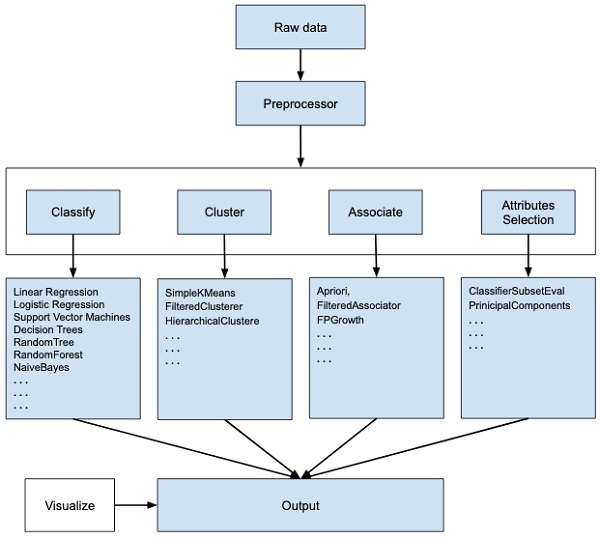
\includegraphics[width=0.75\textwidth]{../img/memoria/weka-summary}
\caption[Resumen de las funcionalidades de Weka.]{Resumen de las funcionalidades de Weka. Imagen recuperada de \url{https://www.tutorialspoint.com/weka/what_is_weka.htm}}\label{fig:whatisweka}
\end{figure}

En la figura~\ref{fig:whatisweka} se observa un diagrama con todas las funcionalidades que ofrece Weka. Para poder utilizar un conjunto de datos en \textit{Machine Learning}, ver sección~\ref{sec:machine-learning}, hay que hacerlos aptos, esto se consigue con el primer paso, el pre-procesado, para ello Weka proporciona una serie de herramientas que permiten limpiar los valores nulos, campos irrelevantes, etcétera. Seguidamente se guardan los datos que han sido pre-procesados en almacenamiento local para aplicar algoritmos de \textit{Machine Learning}\footnote{Esta es una de las principales desventajas de Weka, almacena el conjunto de datos en su totalidad en memoria del sistema, limitando el número de instancias que puede tener un conjunto de datos.}.

En función de qué tipo de modelo de ML se desee aplicar, se selecciona una opción de entre: clasificación, agrupamiento, asociación, o selección de atributos. Weka proporciona una serie de algoritmos para cada modelo, permitiendo su completa parametrización individualizada, de forma que se pueden realizar los experimentos al gusto del investigador. 

Finalmente Weka proporciona un resultado estadístico del procesamiento del modelo, junto con ello proporciona una herramienta de visualización para inspeccionar los datos. Los distintos modelos pueden aplicarse al mismo conjunto de datos, permitiendo la comparación de los resultados.

Página web de la herramienta: \url{https://waikato.github.io/weka-wiki/}

\subsection{PyCharm}

PyCharm es uno de los IDEs\footnote{Entorno de desarrollo integrado, sistema de software para el diseño de aplicaciones que combina herramientas comunes para desarrolladores en una sola interfaz gráfica.} con soporte para Python más completos y exhaustivos, convirtiéndolo en uno de los más populares IDEs. Este éxito proviene en gran medida de que la empresa desarrolladora de este \textit{software} es JetBrains, el desarrollador detrás del popular IDE Intellij IDEA, uno de los 3 IDEs más grandes de Java.

Disponible como una aplicación multiplataforma, PyCharm es compatible con los siguientes sistemas operativos: Windows, Linux y MacOS. Proporciona soporte para las versiones de Python 2.x (descontinuada desde 2021) y 3.x. Provee de un elevado número de módulos, paquetes y herramientas diseñadas para optimizar el desarrollo del código, al mismo tiempo que reduce el esfuerzo necesario para ello. Siendo totalmente personalizable en función de los requisitos de desarrollo y las preferencias personales. Cuenta con:
\begin{itemize}
\item \textit{Debugger} gráfico.
\item Validación de pruebas unitarias.
\item Soporte integrado para sistemas de control de versiones, VCS.
\item Soporte para análisis de datos con Anaconda.
\end{itemize}
PyCharm permite trabajar con múltiples bases de datos directamente sin necesidad de utilizar terceras aplicaciones en forma de intermediarias. A pesar de que está diseñado para Python, tiene soporte para HTML, CSS, Javascript,\dots

Características y ventajas de PyCharm:
\begin{itemize}
\item Editor de código inteligente. 
\item Permite integrar nuevas herramientas.
\item Soporte integrado para \textit{Machine Learning} y \textit{Data Science}.
\item Soporte integrado para Google App Engine.
\item Sistema de \textit{debugging} y \textit{testing}.
\item Soporte para desarrollo de múltiples lenguajes.
\item Navegación a través del código y del proyecto.
\item \textit{Refactoring}.
\item Soporte para desarrollo remoto.
\item Soporte de los principales \textit{frameworks} de desarrollo web.
\item Sistemas de versión de control.
\item Generación de código específico de un lenguaje.
\item Documentación directa de la API en uso.
\item Plantillas para nuevos ficheros.
\item Plantillas <<vivas>>.
\item Ayuda para la importación de bibliotecas.
\item Corrección y optimización del código.
\end{itemize}

Entre las principales desventajas se encuentran:
\begin{itemize}
\item Requisitos mínimos elevados. 
\item Precio de la licencia de uso elevado.
\item Curva de aprendizaje.
\end{itemize}

Página web de la herramienta: \url{https://www.jetbrains.com/pycharm/}

\subsection{\TeX Maker}
\TeX Maker es un \textit{software} multiplataforma, disponible en Windows, Linux y MacOs; el cual permite la edición de documentos \LaTeX. Integra en él todas las herramientas necesarias para la creación, modificación y desarrollo de documentos escritos en \LaTeX. Entre sus características principales destacan el soporte a unicode, comprobación ortográfica <<en directo>>, sugerencias y principalmente un visor del fichero pdf que se está editando. Además en caso de haber errores en la compilación, posee registros indicando el error y la línea que lo ha producido, facilitando el \textit{debugging}.

Añadido a todas las ventajas que oferta, es completamente gratuito.

Página web de la herramienta: \url{https://www.xm1math.net/texmaker/}

\subsection{FileZilla}
FileZilla es un \textit{software} multiplataforma, disponible en Windows, Linux y MacOs; totalmente gratuito, el cual incluye funcionalidades del protocolo FTP. Permite cargar y descargar archivos desde y hacia un servidor, siendo la opción líder en el mercado si se desean hacer múltiples transferencias manteniendo un elevado rendimiento. Ofrece soporte a FTP, SFTP, proveedores \textit{cloud} (Google Drive, OneDrive, Amazon S3 y DropBox). Como característica diferenciadora a otros programas similares, da soporte tanto a IPv4 como a IPv6. 

Además, puede utilizarse como servidor FTP, siendo compatible con HTTP/1.1, SOCKS5, y FTP proxy. 


Página web de la herramienta: \url{https://filezilla-project.org}

\subsection{GitKraken}
GitKraken es un potente \textit{software} diseñado para realizar de forma gráfica todas aquellas tareas que serían realizadas mediante Git en la consola de comandos tradicional. Es una herramienta multiplataforma, con soporte para Windows, Linux y MacOS; permite de forma sencilla mantenerse al tanto de repositorios, \textit{braches}, etiquetas, históricos, realizar \textit{commits}, etcétera. Entre sus características más relevantes destacamos:
\begin{itemize}
\item Soporte para múltiples perfiles.
\item Integración nativa con GitHub Enterprise, GitLab, Bitbucket y VCTS.
\item Edición y visualización de ramas, \textit{merging}, histórico de \textit{commits}.
\item Simplicidad en cuanto a las acciones \textit{merge}, \textit{rebase} y \textit{push}. También admite crear, clonar y añadir repositorios de forma remota, así como ver y crear \textit{pull requests}.
\item Creación de repositorios, favoritos, organización de productos y grupos.
\item Incluye editor \textit{buit-in} de código. 
\item Muestra la diferencia entre los ficheros con cambios respecto a lo ya cometido.
\item Soporte de Gitflow, Git Hooks y LFS.
\end{itemize}

Página web de la herramienta: \url{https://www.gitkraken.com}

\subsection{ZenHub}
ZenHub es una herramienta de gestión de proyectos ágiles integrados en GitHub. Acerca la gestión de proyectos al código, reduciendo los cambios de contexto y aumentando la productividad del equipo de desarrollo. Permitiendo la interconexión de múltiples repositorios en un solo \textit{Workspace}, lo que otorga una visión global de todo el trabajo realizado y por realizar. Ayuda a un equipo de desarrollo a organizar, priorizar, asignar y realizar el seguimiento de las tareas de todo el equipo, adjuntando información estadística y reportes de cada \textit{sprint}.

Se encuentra disponible o como extensión tanto para Google Chrome como para Mozilla Firefox, en sus correspondientes \textit{marketplaces}, o desde la propia página web de ZenHub.

Página web de la herramienta: \url{https://www.zenhub.com}\\

\subsection{Visual Paradigm}
Visual Paradigm es una herramienta UML-CASE: Ingeniería de \textit{Software} Asistida por Computación. Desarrollada para soportar el ciclo de vida completo del proceso de desarrollo \textit{software} a través de la representación de todo tipo de diagramas.

Permitiendo el modelado de modelado de diagramas UML (entre otros), dando soporte principalmente a diagramas de clases, casos de uso,secuencia, estados, actividad, paquetes, etc.

Página web de la herramienta: \url{https://www.visual-paradigm.com/}
\capitulo{5}{Aspectos relevantes del desarrollo del proyecto}

En esta sección se van a detallar los aspectos más relevantes que han ido surgiendo a lo largo del desarrollo del proyecto. Este a sido un desarrollo \textit{software} y como tal ha estado lleno de retos y decisiones técnicas que han tenido que ir tomándose. La formación ha sido un punto de inflexión, sumado a la aplicación de buenas prácticas, ha resultado en un producto de calidad.


\subsection{Investigación}
Uno de los componentes principales que posee el proyecto es el apartado de investigación en el campo del Aprendizaje Automático, concretando un poco más, el efecto de la aplicación de técnicas de selección de instancias en el aprendizaje semi-supervisado.

Uno de los principales retos a los que el autor se ha enfrentado en una primera instancia ha sido adquirir una rápida capacidad de lectura y asimilación de documentación científica, si bien el idioma (inglés) no ha supuesto una barrera, el no poseer experiencia en realizando estas tareas  generó una necesidad que tuvo que ser solventada poco a poco. En los últimos meses del proyecto la agilidad ya estaba ahí, resultando en tareas más fluidas y veloces.

\subsection{Metodología SCRUM}
Como ya se mencionó en la Sección~\ref{SCRUM}, el proyecto se ha realizado siguiendo una metodología ágil, permitiendo trabajar en \textit{sprints} de manera que el trabajo de cada \textit{sprint} se encuentre correctamente fundamentado al inicio de cada uno, permitiendo trabajar con una mayor eficiencia, priorizar el trabajo en función las tareas existentes, y disponer de versiones funcionales a la vez que se sigue con el desarrollo del proyecto.

Si bien se conocía SCRUM de manera puramente teórica, el haber trabajado siguiendo esta metodología ha permitido ganar experiencia en modelos de desarrollo ágiles, diferente de los clásicos a los que se acostumbraba, y tal y como se define, el trabajo se ha visto afectado de forma positiva con esta aproximación.

Se disponían de cerca de 9 meses (máximo) para cumplimentar el proyecto, un tiempo mucho más elevado del habitual para este tipo de proyectos, es por ello que se han invertido múltiples \textit{sprints} para validación y calidad, permitiendo asegurar que los pasos dados son correctos y seguir construyendo sobre seguro.

Una de las principales dificultades encontradas en este campo es la asignación de puntos de historia, el definir en base a un nombre de tarea y una descripción el tiempo que va a ser necesario invertir para cumplir con ella no ha sido siempre muy preciso. El no poseer experiencia previa en proyectos de esta envergadura propició que se considerara la equivalencia de 1 punto de historia igual a 45 minutos o menos. Y si bien ha habido múltiples \textit{sprints} en los cuales se ha conseguido seguir esta relación, no ha sido algo lineal en el proyecto, debido a que se tuvo en cuenta la experiencia que se iba consiguiendo a la hora de asignar los siguientes puntos de historia, y ha habido múltiples \textit{sprints} desfasados por lo alto.

\subsection{Actualización y modificación de un \textit{software} pre-existente}
Posiblemente será el aspecto relevante más cercano a el futuro laboral de cualquier alumno. Supuso todo un reto el coger un proyecto que había sido desarrollado por 5 personas y <<hacerlo propio>>. Como es lógico cada persona programa de una forma diferente para alcanzar la misma funcionalidad, y ya no solo eso, sino la propia temática del proyecto era desconocida, por lo tanto supuso un esfuerzo doble.

La no existencia de una documentación, ni técnica ni formal, acerca del propio \textit{software} no ayudó a obtener una visión del proyecto más allá de la estructura de paquetes y nombres. Fue algo que se echó en falta, y que con la finalización de este proyecto, ya posee.

\subsection{Desarrollo Web}
A lo largo del Grado no se ha impartido docencia en cuanto a desarrollo web se refiere, siendo toda una desventaja a la hora de actualizar y modificar \texttt{UBUMLaaS}. Trabajar con una REST API era algo hasta enero desconocido, y la curva de aprendizaje no ha sido especialmente sencilla. Han sido necesarias numerosas horas para familiarizarse tanto con el proyecto como con la forma de trabajo que poseen las aplicaciones que siguen esta arquitectura.

A la hora de integrar nuevas modificaciones sobre el \textit{backend} del proyecto no supuso grandes problemas, fue un trabajo laborioso como es de esperar, pero al ser Python ya se estaba acostumbrado al lenguaje de programación. La dificultad llegó con el \textit{frontend} lenguajes de marcas como HTML o CSS, y de programación como JavaScript, no eran desconocidos, pero no se habían utilizado nunca en grandes proyectos; es por ello que hubo tareas que se vieron retrasadas. 

Destacar que como ha sido la tónica general del proyecto, y así queda recogido en el resumen de numerosos \textit{sprints} en su anexo correspondiente, a medida que el equipo de desarrollo se familiarizaba con el lenguaje y entorno de aplicación, la velocidad de implementación de funcionalidades crecía de forma exponencial.

La web ha sufrido una renovación completa, siendo necesario re-escribir todos los documentos HTML, si bien se tuvo desde un inicio en cuenta que ciertas páginas tuvieran un diseño similar al que ya poseían anteriormente para seguir con el diseño inicial. El nuevo diseño soporta múltiples resoluciones de pantalla, habiendo sido priorizadas aquellas soportadas en tabletas sobre las de dispositivos móviles.

\subsubsection{Funcionalidades <<sobre la marcha>>}
En el momento de desarrollo de la parte de administración de \texttt{UBUMLaaS} surgían cada día nuevas funcionalidades que parecían correctas o adecuadas para implementar y añadir, permitiendo a los administradores tener más control del que iban a poseer una vez pase a producción la versión creada.

Muchas de estas nuevas funcionalidades se han llevado a cabo y se encuentran disponibles y completamente integradas con la plataforma, si bien muchas otras no, se han quedado como trabajos futuros. Aquellas que se han quedado sin implementar fueron clasificadas con una relevancia baja, siendo priorizadas aquellas que se consideraron más útiles o curiosas.

\subsection{PIP}
\texttt{IS-SSL} es una biblioteca desarrollada con la finalidad de que sea útil a la mayor cantidad de desarrolladores posible, siguiendo las directrices del \textit{Open Source}, es por ello que se encuentra disponible a través del gestor de paquetes de Python, PIP. 

El proyecto también puede ser descargado directamente desde el repositorio de GitHub y realizar todas las instalaciones de dependencias necesarias a través del fichero de \textit{requeriments.txt} o creando un entorno de \texttt{Conda} (a través del fichero \textit{is-ssl.yml}).

\subsection{Docker}
\texttt{UBUMLaaS} se encuentra desplegado en la Universidad de Burgos sobre un servidor directamente, pero con el fin de permitir que se despliegue en cualquier equipo y que la configuración específica sea mínima, se ha creado un contenedor Docker en el cuál reside la última versión de la aplicación. 

El futuro de la aplicación podría ser únicamente en Docker perfectamente, siendo mucho más sencillo desplegarla en diferentes servidores, pero en la actualidad ese no es el enfoque deseado, por lo que se dejó para hacer al final en caso de que sobrara tiempo, como ha sucedido.

\subsection{Validación de la integridad de los algoritmos implementados}
Todos los algoritmos los cuáles se encuentran disponibles en \texttt{IS-SSL} han sido validados y refinados a lo largo de múltiples iteraciones de trabajo con el fin de garantizar su integridad, de forma que se puede asegurar que reportan resultados tal y como el \textit{paper} original lo presentó.

\begin{itemize}
\item Los algoritmos de selección de instancias han sido validados contra los homónimos correspondientes proporcionados por \texttt{Weka}, \textit{software} de ML desarrollado por la Universidad de Waikato.
\item Los algoritmos de aprendizaje semi-supervisado han sido validados contra los implementados por el grupo de investigación ADMIRABLE de la Universidad de Burgos.
\end{itemize}


\subsection{Experimentación de filtros de ruido para aprendizaje semi-supervisado}
\imagenFlotante{../img/memoria/aspectos-relevantes/General}{Resumen en función del clasificador y filtro.}{exp-general}

\capitulo{6}{Trabajos relacionados}

Entre los trabajos relacionados con este Trabajo de Fin de Grado, se distinguen las bibliotecas y \textit{frameworks} enfocadas en \textit{Machine Learning} y los \textit{Machine Learning as a Service} (MLaaS) más relevantes.

\section{\textit{Frameworks} y bibiotecas}\label{related:frameworks}
Aunque está categorizado con dos términos, se puede entender un \textit{framework} de \textit{Machine Learning} como una herramienta, librería o interfaz que proporciona a los desarrolladores facilidades para crear modelos de aprendizaje automático.

\begin{enumerate}
\item \textit{\textbf{Scikit-Learn}.}
Coloquialmente conocido como <<Sklearn>>, es la librería más útil y robusta para aprendizaje automático implementada en Python. Se trata de un \textit{software open source}. Entre la multitud de algoritmos que provee, destacan varios para problemas de clasificación, regresión y \textit{clustering}; incluyéndose además máquinas de soporte vectorial (SVM), \textit{random forests}, \textit{gradient boosting}, \textit{k-means} y DBSCAN.

A pesar de estar escrito en su mayor parte en Python, y el uso que le da a la librería de NumPy\footnote{Librería de Python que da soporte al uso de vectores y matrices con una gran dimensionalidad. Además proporciona una gran colección de funciones matemáticas de alto nivel para operar con ellas.} para el cálculo de operaciones algebraicas en entornos de alto rendimiento, el \textit{core} de la librería está escrito en Cython para mejorar el rendimiento. 

\item \textbf{\textit{Tensor Flow}.}
Bajo el desarrollo de Google, es una biblioteca \textit{open source} para computación numérica, utiliza gráficos de flujo de datos. En las gráficas los nodos representan operaciones matemáticas mientras que los bordes representan las matrices de datos multidimensionales.

Mediante su arquitectura flexible permite la implementación del cálculo en una o varias CPU o GPU, en servidores, o equipos móviles, todo con una sola API\footnote{Conjunto de definiciones y protocolos que se utiliza para desarrollar e integrar el \textit{software} de  las aplicaciones, permitiendo la comunicación entre dos aplicaciones a través deun conjunto de reglas.}. Su diseño esta principalmente enfocado para la resolución de problemas mediante redes neuronales, pero es lo suficientemente general como para ser aplicable a una amplia variedad de dominios.

\item \textbf{\textit{Torch}.}
Marco de cálculo científico con amplio soporte para algoritmos de aprendizaje automático el cual da prioridad al uso de GPU sobre CPU, se trata de un \textit{software open source}. Una de sus características principales es el rendimiento y eficiencia que proporciona, esto se debe a que escrito en LuaJIT y una implementación subyacente de C/CUDA.

\item \textbf{\textit{Theano}.}
Librería de Python la cual da soporte a la definición  de expresiones matemáticas empleadas en aprendizaje automático, la optimzación de estas expresiones y la evaluación de la eficiencia con el uso de GPU. Siendo capaz de rivalizar implementaciones escritas en C. Theano está distribuida bajo licencia BSD\footnote{Licencia de \textit{software} libre permisiva, de igual manera que la licencia MIT, posee menos restricciones que GPL, siendo muy cercana al dominio público.}.

\item \textbf{\textit{Veles}.}
Escrito en C++, sus aplicaciones se encuentran dentro del marco del aprendizaje profundo. A pesar de ello utiliza Python para la automatización y coordinación de sus nodos. Sus objetivos principales son la flexibilidad y el rendimiento. Permitiendo la normalización de los datos antes de introducirlos en un cluster.

Veles permite entrenar redes convolucionales, redes recurrentes, redes totalmente conectadas y otras topologías populares.

\item \textbf{\textit{H2O}.}
Marco de aprendizaje automático, \textit{open source}. Orientado principalmente a negocios, implementa análisis predictivo para ayudar a la toma de decisiones basadas en datos y conocimientos. Proporciona herramientas únicas como el soporte agnóstico de bases de datos, una interfaz WebUI. 

H2O provee de modelos y soporte para Python, R, Java, JSON, Scala, JavaScript. Su \textit{core} está escrito en Java.

\end{enumerate}

\section{\textit{Machine Learning as a Service}}\label{related:MLaaS}
El Aprendizaje Automático como servicio (MLaaS por sus siglas en inglés), es una tecnología de aprendizaje automático que es habitualmente adquirida de un tercero. Su funcionamiento es similar a SaaS (\textit{Software as a Service}) o PaaS (\textit{Platform as a Service}), i.e. un usuario utiliza los servicios de una empresa en lugar de los suyos propios.

\begin{enumerate}
\item \textbf{\textit{Amazon Machine Learning}.}
Servicio ofrecido por Amazon el cual proporciona todas las herramientas necesarias para utilizar modelos de aprendizaje automático sin necesidad de conocer todos los detalles y configuraciones de estos. No quedándose ahí, proporciona herramientas de análisis de datos y modelos pre-entrenados para casos de uso habituales como detección de fraude en aplicaciones móviles.

Encaja a la perfección con proyectos o necesidades que necesitan interacción en tiempo real. A pesar de que únicamente proporciona soporte a problemas de clasificación binaria o multi-etiqueta, y regresión; posee la potente funcionalidad de que es el propio servicio el que decide qué algoritmo utilizar para el problema dado.

\item \textbf{\textit{SageMaker}.}
Entorno de aprendizaje automático con el objetivo de simplificar el trabajo a los científicos de datos, para ello proporciona herramientas que permiten la creación y despliegue de forma rápida de modelos.

Proporciona multitud de modelos que su predecesor (Amazon \textit{Machine Learning}) no poseía, como es el caso del aprendizaje no supervisado. Siendo la evolución natural para aquellas empresas que ya utilizan los servicios web de Amazon (AWS).

\item \textbf{\textit{Microsoft Azure AI Platform}.}
Proporciona una plataforma unificada con todas las API correspondientes a técnicas de aprendizaje automático y servicios de infraestructura en Azure.

Destaca \textit{Azure Machine Learning} como entrono por excelencia para el manejo de conjuntos de datos, creación, entrenamiento y despliegue de modelos. Permitiendo que desde la interfaz web y con muy poca codificación necesaria, se puedan crear modelos. Ofreciendo soporte a cerca de cien métodos para problemas de clasificación binaria y multi-etiqueta, detección de anomalías, regresión, recomendación, análisis de textos, y como único algoritmo de \textit{clustering}, \textit{k-means}.

\item \textbf{\textit{Google Cloud ML}.}
Plataforma de \textit{Machine Learning} basada en la nube que sugiere un enfoque sin código para construir soluciones basadas en datos. Fue diseñado para que tanto los recién llegados como los ingenieros fueran capaces de construir modelos personalizados. Como es habitual, ofrece también un conjunto de modelos pre-construidos, a través de un conjunto de API.

\item \textbf{\textit{IBM Watson Machine Learning Studio}.}
Aporta una interfaz de procesamiento de datos y creación de modelos totalmente automatizada que apenas necesita formación para empezar a procesar los datos, preparar los modelos y desplegarlos en producción.

La parte automatizada es capaz de resolver problemas de clasificación binaria y multi-etiqueta, y regresión. Permitiendo la opción de que el usuario elija el modelo de \textit{Machine Learning} deseado o que sea el propio sistema el que infiera el que considera mejor a partir de los datos. 

\end{enumerate}
\capitulo{7}{Conclusiones y Líneas de trabajo futuras}

En esta última sección se exponen las conclusiones finales recuperadas del proyecto realizado. Además, se añaden las líneas futuras que se pueden seguir para continuar con el desarrollo de las bibliotecas, y/o de \texttt{UBUMLaaS}.

\section{Conclusiones}
Conclusiones a las que se llega posterior al desarrollo del proyecto.

\begin{itemize}
\item Los objetivos del proyecto han sido cumplidos satisfactoriamente.
	\begin{itemize}
	\item \texttt{IS-SSL}. Ahora la comunidad cuenta con dos bibliotecas las cuales proporcionan aquellos algoritmos más comúnmente utilizados en la literatura. Estas son públicas permitiendo que cualquier persona pueda utilizarlas.
	\item \texttt{UBUMLaaS.} La aplicación cuenta con soporte para algoritmos de aprendizaje semi-supervisado. Además dispone de una <<parte>> de administración la cuál va a permitir a los usuarios con el rol de administrador ser capaces de no solo conocer el estado del sistema, sino también administrar usuarios y poseer estadísticas en tiempo real, todo ello sin necesidad de acceder a la base de datos <<a mano>>.\\
	Tras la finalización del proyecto, \texttt{UBUMLaaS} cuenta con una documentación técnica de programador, lo cual favorecerá su evolución y desarrollo futuro, así como la facilidad de mantenimiento y reducción de deuda técnica.
	\end{itemize}
\item La lectura de artículos científicos ha sido algo totalmente nuevo, siendo necesarias numerosas horas para su interpretación (sobretodo en los primeros), se debe destacar que según se avanzaba en el desarrollo del proyecto, la familiarización con éstos ha sido satisfactoria, permitiendo asimilar e implementar los algoritmos deseados con mayor facilidad.
\item El haber desarrollado los algoritmos de \texttt{IS-SSL} en Python posee las ventajas de poseer multitud de bibliotecas orientadas a operaciones vectoriales y con \textit{DataFrames}, su portabilidad, posee una baja curva de aprendizaje, y que se trata de un lenguaje de alto nivel.
\item Las bibliotecas poseen una estructura que permite su escalabilidad, permitiendo que no sea un trabajo cerrado sino que se puedan ampliar y seguir evolucionando.
\item El desarrollo de \texttt{UBUMLaaS} ha permitido ampliar el número de tecnologías conocidas, en un inicio se habían utilizado muy poco la mayor parte de las tecnologías utilizadas para el desarrollo del \textit{frontend}. Pero a la hora de finalizar el trabajo ya se está familiarizado con ello y se posee una confianza y capacidades de desarrollar garantizando una calidad dada.
\item A lo largo del desarrollo del proyecto se han utilizado diferentes herramientas \emph{cloud}, éstas han permitido aumentar la calidad del producto final que se iba obteniendo en sucesivas iteraciones. Se deberían de haber definido en un primer momento antes de comenzar a desarrollar el proyecto, pero algunas de ellas eran desconocidas. Cabe destacar que el esfuerzo extra que ha tenido que ser invertido, en futuros proyectos resultará útil.
\end{itemize}

Como \textbf{conclusión final}, destacar la oportunidad de \emph{aprendizaje} que el desarrollo de este proyecto ha supuesto. Desde el minuto uno se ha requerido dominar ciertas tecnologías vistas (y nuevas) a lo largo de todo el Grado, incluso a la hora de escribir la documentación. El número de horas que el proyecto iba a requerir se conocía desde un primer momento pero el razonamiento inicial de \emph{<<quedan 8 meses por delante, hay tiempo para todo>>}, si bien se ha cumplido (el proyecto se ha terminado antes de las fechas de entrega), la disciplina de trabajo como si fuera un entorno laboral ha sido necesaria.

\section{Líneas de trabajo futuras}

\textbf{\texttt{UBUMLaaS}}, dada la morfología y arquitectura de la aplicación, existen numerosas opciones de mejora o líneas de trabajo futuras.
\begin{itemize}
\tightlist
\item Migración de la aplicación a \texttt{Kubernetes}, permitiendo el despliegue sobre \textit{clusters}. Dada la naturaleza de la aplicación, es una evolución lógica.
\item Aumentar el número de algoritmos soportados, incluyendo su implementación en diferentes lenguajes (actualmente soportados \texttt{IS-SSL}, \texttt{Scikit-Learn} y \texttt{Weka}).
\item Aumentar el conjunto de pruebas de forma que abarquen tanto \textit{backend} como \textit{frontend}.
\item Realizar un proceso de refactorización (únicamente en caso de que el proyecto vaya aumentar sus funcionalidades).
\item Mejoras de \textit{backend}:
	\begin{itemize}
	\tightlist
	\item Soporte de parseo de ficheros mediante URL.
	\item Soporte de parseo de ficheros personalizados (separadores, saltos de línea, etc.).
	\item Detección de entrenamientos idénticos repetidos con el fin de evitar repetir procesos demasiado largos en CPU.
	\item Migración de la ejecución de los entrenamientos a ejecución en GPUs.
	\item Proporcionar soporte de ejecución paralela sobretodo en aquellos procesos con validación cruzada.
	\end{itemize}
\item Mejoras de \textit{frontend}:
	\begin{itemize}
	\tightlist
	\item Añadir un modo oscuro a la aplicación.
	\item Soportar la descarga de históricos y estadísticas, tanto del estado del sistema como de los experimentos en ejecución.
	\item Separar el perfil del usuario con sus estadísticas personales, de los conjuntos de datos y experimentos asociados al mismo.
	\item Permitir el auto-refresco de la vista cuando un usuario se quede <<esperando>> a que el experimento finalice.
	\end{itemize}
\end{itemize}

\textbf{\texttt{IS-SSL}}, el propio diseño de ambas bibliotecas sugiera una posible unión en el futuro, en caso de que se acaben comenzando a utilizar de forma conjunta y facilite su uso. 

Para facilitar la aportación de la comunidad a las bibliotecas, se van a definir las convenciones, buenas prácticas, \ldots de forma que la evolución de las bibliotecas mantenga una estructura y un código limpio y sobretodo, \emph{fácil} de mantener. En esta misma línea se va a aplicar el método plantilla~\cite{shvets2021} con el fin de re-estructurar las bibliotecas, permitiendo crear un \texttt{core} común y desacoplar ciertas funcionalidades.

Una de las mejoras que se plantean para realizar a corto/medio plazo es la migración de los algoritmos a \texttt{Cython}, de manera que haya un aumento considerable del rendimiento. Otra opción que se propone es la modificación de los algoritmos para, en aquellas partes soportadas, corran en paralelo tanto mediante hilos, como mediante procesadores lógicos o reales.

\textbf{Investigación.} La investigación, como es lógico, no está ni cerca de estar terminada. El campo es muy amplio y quedan muchas preguntas por responder. Una de las principales mejoras que se puede realizar es hacer uso de \textit{Random Forests} en lugar de árboles de decisión, evitando que queden hojas con una única instancia y afecten a la clasificación en el aprendizaje semi-supervisado~\cite{tanha2017semi}.




\bibliographystyle{plain}
\bibliography{bibliografia}

\end{document}
